\documentclass[review,11pt]{elsarticle}
%\documentclass[preprint,review,12pt,authoryear]{elsarticle}
\usepackage{lineno,hyperref,ulem,todonotes}
\usepackage{rotating}
\usepackage{amsmath}
\modulolinenumbers[5]
%\usepackage{natbib}
\usepackage{tabularx,ragged2e,booktabs,caption}
\journal{Computational Geosciences}

\usepackage{placeins}
%%%%%%%%%%%%%%%%%%%%%%%
%% Elsevier bibliography styles
%%%%%%%%%%%%%%%%%%%%%%%
%% To change the style, put a % in front of the second line of the current style and
%% remove the % from the second line of the style you would like to use.
%%%%%%%%%%%%%%%%%%%%%%%

%% Numbered
\bibliographystyle{model1-num-names}

%% Numbered without titles
%\bibliographystyle{model1a-num-names}

%% Harvard
%\bibliographystyle{model2-names.bst}\biboptions{authoryear}

%% Vancouver numbered
%\usepackage{numcompress}\bibliographystyle{model3-num-names}

%% Vancouver name/year
%\usepackage{numcompress}\bibliographystyle{model4-names}\biboptions{authoryear}

%% APA style
%\bibliographystyle{model5-names}\biboptions{authoryear}

%% AMA style
%\usepackage{numcompress}\bibliographystyle{model6-num-names}

%% `Elsevier LaTeX' style
%\bibliographystyle{elsarticle-num}
%%%%%%%%%%%%%%%%%%%%%%%

\begin{document}

\begin{frontmatter}

\title{Simulation Study of a Novel Subgrid Model for Microtopography Effect on Surface Flow}

%\author[ornl]{Ahmad Jan \corref{cor}} \author[lanl1]{Ethan T. Coon} \author[ornl]{Scott L. Painter} \author[lanl2]{Rao Garimella} \author[lanl2]{J. David Moulton}

%\address[ornl]{Climate Change Science Institute and Environmental Sciences Division, Oak Ridge National Laboratory, Oak Ridge, Tennessee, USA\fnref{copyrightnotice}} 
%\address[lanl1]{Computational Earth Sciences Group, Earth and Environmental Sciences Division, Los Alamos National Laboratory, Los Alamos, New Mexico, USA} 
%\address[lanl2]{Applied Mathematics and Plasma Physics Group, Theoretical Division, Los Alamos National Laboratory, Los Alamos, New Mexico, USA} 


%\cortext[cor]{Corresponding Author: Ahmad Jan; Email: jana@ornl.gov; Phone: (865) 576-8175.}



\begin{abstract}
In permafrost-affected regions, subsurface is mainly characterized by ice-wedge polygons that form a patterned polygonal ground. The role of patterned polygonal ground and the associated fine-scale microtopography (at a scale smaller than the size of polygons) in controlling surface/subsurface thermal hydrology is critical but well-understood. Fine-scale simulations are required to capture microtopographic influences on flow. Standalone fine-scale surface hydrology simulations are feasible with modern computing tools. However, highly resolved integrated surface/subsurface thermal hydrology simulations are not tractable at watershed scale and requires proper modeling. To capture the effects of microtopography (depressions, obstructions etc.) in coarsened model, we present a subgrid model parameterized by fine-scale microtopographic features, which alters the water storage and flow terms in the governing equations. Simulations were carried out and numerical results of the subgrid model were compared both to those generated with no subgrid model and to fine-scale results of seven ice-wedge polygons. Our findings confirm that the subgrid model improves the shape of the hydrographs and the total water content in the system, and that the results are very close to the corresponding fine-scale simulations. Watershed-scale fully integrated surface/subsurface simulations with the subgrid model show that the surface depressions increase infiltration and reduce runoff, thereby highlighting the microtopographic effects on the watershed-scale hydrology. Finally, our work explores how parameters can be deduced from the available fine-scale information to account for microtopographic effects in coarsened integrated models.
%that the model has the potential  to accurately represent fine-scale behavior at larger spatial scales.
\end{abstract}

\begin{keyword}
Subgrid model \sep Permafrost \sep Polygonal tundra \sep  Microtopography  \sep Watershed \sep Integrated Surface/Subsurface
\end{keyword}


\end{frontmatter}

\linenumbers
%Photograph showing the polygonal structure of the field site A, 
\FloatBarrier
\section{Introduction}\label{introduction}
%The widely distributed wedges of ice form a polygonal landscape. 
 %ignoring fine-scale heterogeneity in Arctic landscapes may bias estimates of water head carbon fluxes in large-scale climate and ecosystem models.
The Arctic landscapes are dominated by polygonal patterned (interconnected polygons) ground. The formation of polygonal landscapes in permafrost-affected regions is a consequence of recurring cracks-compression process over hundreds of thousands of years. During winter, vertical fractures are formed due to ground contraction, the water from the snowmelt in the following summer penetrates those cracks and refreezes. In the following winter, the reexpansion of the ice in the cracks compresses the soil horizontally. The recurring crack-compression process over long period of time develops wedges of ice and finally a polygonal landscape is formed~\cite{lachenbruch1962mechanics,greene1963contraction,mackay1990some,mackay2004thermally}. Figure~\ref{ngee-arctic-fieldsites} displays a polygonal tundra, which is a field site of the U.S. Department of Energy's Next Generation Ecosystem Experiments (NGEE) Arctic project located within the Barrow Environmental Observatory (BEO)~\cite{kumar2016modeling}.
\begin{figure}[!h]
\centering
 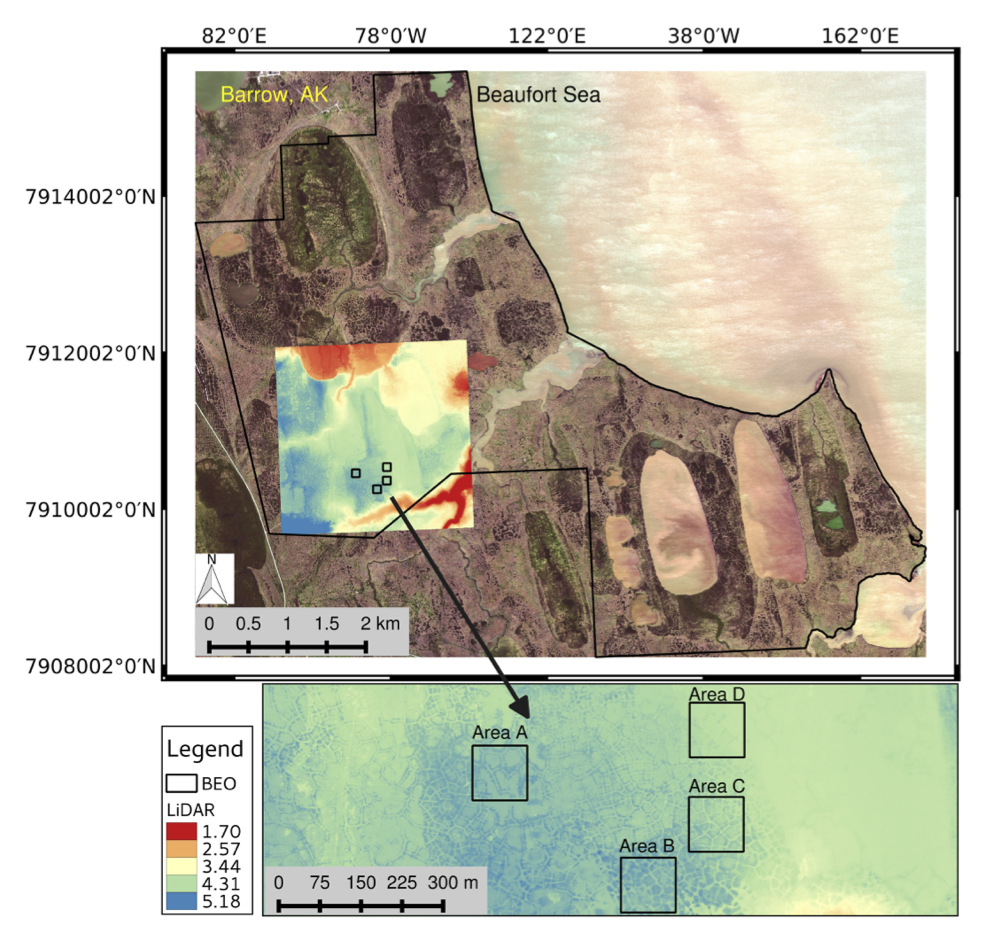
\includegraphics[width=14cm, height=17cm]{./figures/ngee-arctic-fieldsites.png}
\caption{NGEE-Arctic field sites at BEO~\cite{kumar2016modeling}.}
\label{ngee-arctic-fieldsites}
\end{figure}
Several types of polygons are formed due to permafrost degradation. Typically, the polygons are classified as low-centered polygon (LCP) and high-centered polygon (HCP) based on surface microtopography. The LCP has a raised rim and central depression, thereby holds ponded water in the center during the summer that can only be available for infiltration and evaporation. The HCP has elevated center that slopes downward to trough and enhances runoff, thus the center may remain mostly dry. 
Thawing of ice-wedges cause the raised rims of LCP to subside and lead to the formation of HCP~\cite{jorgenson2006abrupt}. The loss of depression storage in the LCP has the ability to connect the disconnected troughs, thus transforms a poorly drained tundra to a well-established drainage network. These changes will potentially alter the entire ecosystem and will bring substantial hydrological changes (e.g., surface/subsurface interactions, distribution of surface water, discharge rate etc.)~\cite{hinzman2005evidence,rowland2010arctic,liljedahl2012ice}.
%--------------------------
To better understand the interactions between surface and subsurface, surface runoff and discharge rate, it is important to gain insight into the role of
heterogeneous spatial structure of the ground surface.
It is well understood that the spatial heterogeneity in the surface microtopography (unevenness at small scale) serves a critical role in the surface water retention, surface/subsurface interactions, and delay runoff, and thereby significantly affects the shape of the hydrographs~\cite{huang2009influences}[\textbf{References}]. In general, an accurate flow representation is achieved at fine-scale (a scale of centimeters) and fortunately with the availability of sophisticated simulation tools, standalone highly resolved surface-flow simulations are easily tractable. However, fully integrated surface/subsurface thermal hydrology simulations with highly resolved computational grid are not tractable at watershed scale. The processes representing flow will not be accurate if the microtopographic effects are ignored in the integrated models. This idea to incorporate fine-scale flow behavior in the watershed-scale integrate models motivates the use of subgrid representation.

Due to the huge computational burden, the effects of spatially varying surface microtopography in watershed-scale integrated surface/subsurface models are typically ignored, and hence the processes representing flow are not accurate. The important challenge to address is: how to capture fine-scale flow behavior in the watershed-scale integrated models. To accomplish this task, the existing hydrological models need to alter
%---------------------------



%, and further how to capture fine-scale flow behavior at larger scales. 

. However, to account for fine-scale behavior at large scales, the model must be able to incorporate fine-scale spatial variability because high-resolved simulations are not tractable at larger spatial and temporal scales. The task of capturing fine-scale flow behavior at larger scales is accomplished by modifying the storage and flow terms in the governing flow equation. This alteration of terms yield subgrid models. 

%The fact that fine-scale simulations are computationally expensive and not tractable at larger scales, effects of spatially varying surface mictopography are usually ignored, hence the processes representing surface flow are not accurate.  
A subgrid model is build on the information gained from highly resolved surface topographic data: the depressions and obstructions. Depressions are disconnected low points in the topography (surface pits) that retain water that is available only for infiltration or/and evaporation. Obstructions are objects exit above the depressions that interrupt and slow the flow, but do not completely block it. The depressions modify the accumulation term and a friction factor (more details below) is used in the flow law to introduce obstructions. 
%To capture these effects in a model, the depressions require to alter the accumulation term and a friction factor need to introduce a friction factor to influence the surface flow term and hence surface detention.

The integrated suface/subsurface modeling has received considerable attention from researchers across the world; see, for example,~\cite{painter2013modeling,kurylyk2014climate,spainter2016integrated} and references therein. Here we focus only on the subgrid modeling approach. Though the concept of microtopographic features and their implications on the flow and discharge is not new, but has not been fully addressed and understood from modeling perspective. Accurate representation of surface microtopography in a coupled surface/subsurface hydrologic model at watershed-scale is a challenging task. 
% -----------------------------------------------------------------------------------------------------------------------------------------------------------------------------------
In the mid-1950s, the significance of the surface microtopographic features were described in~\cite{stammers1956effect}. 
A one-dimensional simulations to study the effects of spatially varying surface roughness on flow hydrographs is presented in ~\cite{huang2009influences}
Panday and Huyakorn (\citeyear{panday2004fully}) presented an integrated surface/subsurface flow model with subgrid representation through the surface depressions and obstructions by modifying the overland flow governing equation. \textbf{INCOMPLETE!!}
%-----------------------------------------------------------------------------------------------------------------------------------------------------------------------------------------------

The rest of the paper is organized as follows. Section~\ref{subgridmodel} introduces the derivation of the governing equations of the subgrid model. A short description, for a quick reference, of the Advanced Terrestrial Simulator (ATS) and the Arcos multiphysics management framework, within which we implemented our subgrid model, is presented in Section~\ref{ATS}. In Section~\ref{numerical-tests} we compare the numerical results of our subgrid model with no subgrid model and fine-scale results to illustrate the accuracy of our subgrid model for capturing fine-scale microtopographic features. Finally, in Section~\ref{conclusion}, we offer closing remarks and future research inline with thaw-induced subsidence.



\section{Subgrid Model}\label{subgridmodel}
This section describes the derivation of the subgrid model. The subgrid model alters the accumulation term and the flow law. For example, the ponded depth in the accumulation term is typically replaced with a volumetric depth, the ponded depth that would occur if the surface were flat. Specifically, we make the substitution in the accumulation term, where is ponded depth. The volumetric head may be calculated on geometric arguments. Specifically, if the microtopographic elevation field on an ice-wedge polygon (IWP) is $Z_*(x,y)$, the the volumetric depth is
\begin{equation}\label{volumetric-depth1}
\Phi (\delta) = \frac{1}{A} \iint \left( \delta + Z_0 - Z_*(x,y) \right ) H \left( \delta + Z_0 - Z_*(x,y) \right ) dx dy
\end{equation}
Where the integration is over the surface of the IWP, $A$ is the area of the IWP, $Z_0$ is the minimum elevation in the IWP, and $H$ is the Heaviside function. This could be computed from the microtopography and stored as a lookup table. Or, we could employ a simpler parameterization. To that end, we consider parameterizing the microtopography with two parameters: (1) the elevation range spanned by the subgrid microtopography $\delta_\text{max}$, and (2) the specific excluded volume $\delta_\text{ex}$, which is the soil volume per unit bulk area. Then, we approximate the volumetric depth as

\begin{equation}\label{volumetric-depth2}
\Phi (\delta) =
\begin{cases} (2 \delta_\text{max} - 3 \delta_\text{ex}) \left(\frac{\delta}{\delta_\text{max}} \right )^2 + (2 \delta_\text{ex} -  \delta_\text{max}) \left(\frac{\delta}{\delta_\text{max}} \right )^3 & \text{if} \hskip 0.1in 0 \leq \delta \leq \delta_\text{max}, \\
\delta - \delta_\text{ex} & \text{if} \hskip .1in \delta > \delta_\text{max}.
\end{cases}
\end{equation}
The IWP shown in Fig~\ref{3Dpolygon40} was used to evaluate the parameterization Equation~\ref{volumetric-depth2}. The volumetric depth calculated from the approximation Equation~\ref{volumetric-depth2} is compared (curve) with the direct calculation Equation~\ref{volumetric-depth1} (dots) for an ice-wedge polygon in Figure~\ref{polygons}. Also, shown is the volumetric depth in the absence of microtopography, which is linear with slope unity. Equation~\ref{volumetric-depth1} is a very good approximation.
Microtopographic effects on the flow law are not as straightforward to incorporate as the volumetric head $\Phi(\delta)$. In particular, we should make the distinction between depressions and obstractions (Panday and Huyakorn, 2004). Depressions are disconnected low points in the topography. The ponded depth must rise above the level of those depressions before any flow can happen. Obstructions exist above the depressions and interrupt and slow the flow, but do not block it completely.
To model the effects of obstructions and depressions, we propose the following modification to the flow law
\begin{equation}
U = - \Theta(\delta) \frac{(\delta - \delta_\text{d})^{2/3}}{n_\text{mann} (\| \nabla Z \| +\epsilon)^{1/2}}
\end{equation}
where $\delta_\text{d}$ is the depression depth, and $\Theta(\delta) \in [0,1]$ is a fractional conductance which account for flow reduction by obstructions.
polygons-finescale
\begin{figure}
\centering
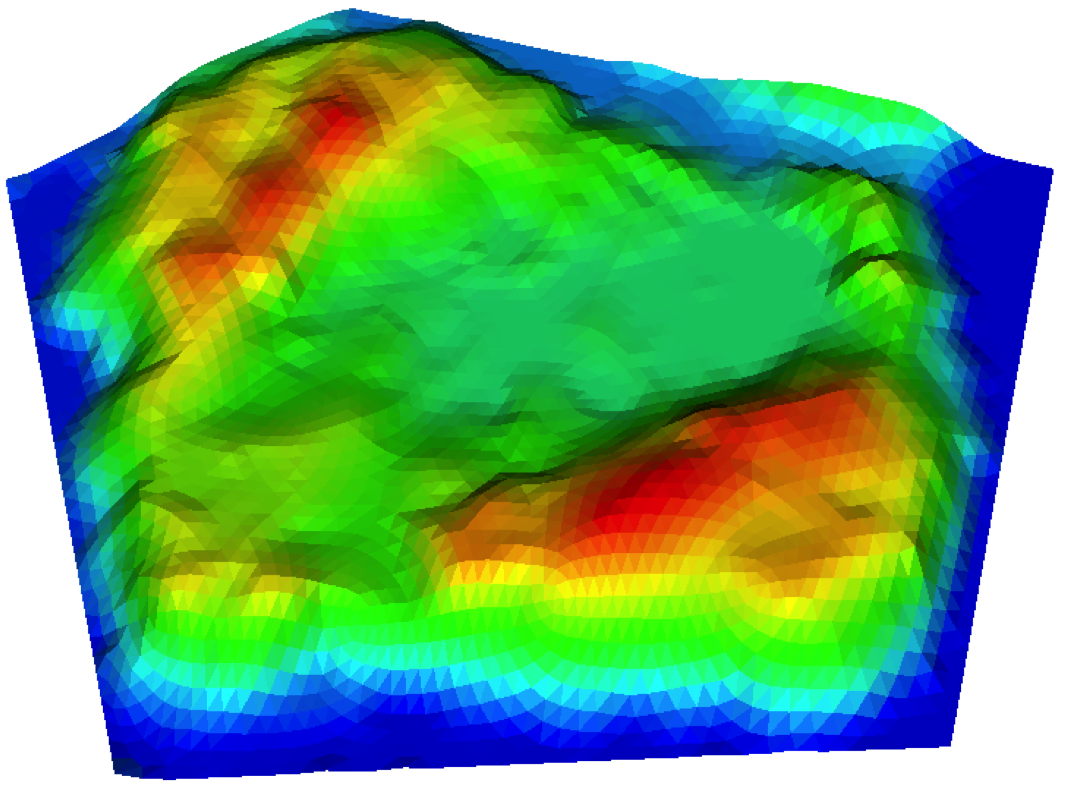
\includegraphics[width=11cm, height=6cm]{./figures/polygons-finescale/3Dpolygon40.png}
\caption{Microtopograpy for an example ice-wedge polygon from the Barrow Environmental Observatory (BEO).}
\label{3Dpolygon40}
\end{figure}

\begin{figure}
\centering
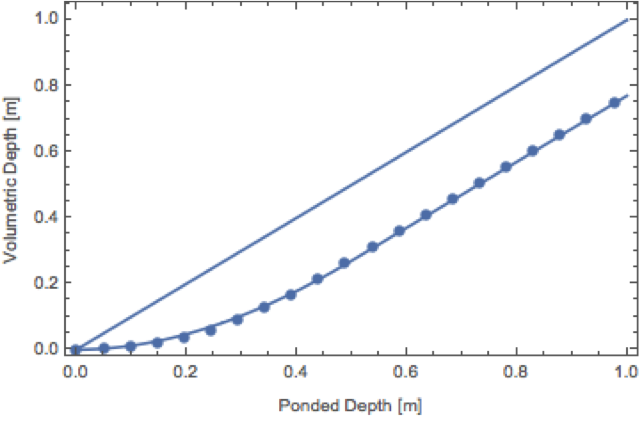
\includegraphics[width=12cm, height=8cm]{./figures/polygons-finescale/polygon40.png}
\caption{Volumetric depth versus ponded depth for polygon shown in Figure~\ref{3Dpolygon40}.}
\label{polygon40}
\end{figure}

\begin{figure}
\centering
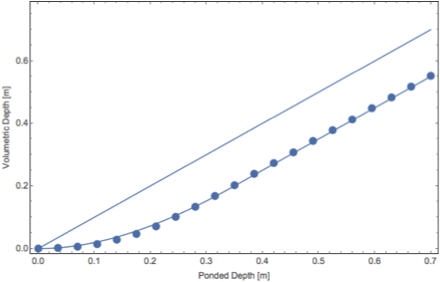
\includegraphics[width=6cm, height=6cm]{./figures/polygons-finescale/picture2.png}
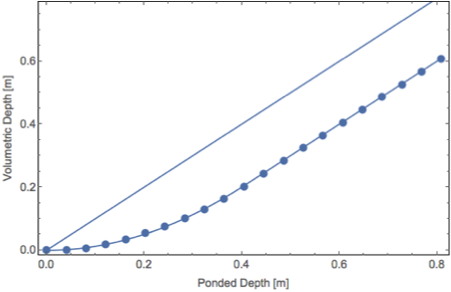
\includegraphics[width=6cm, height=6cm]{./figures/polygons-finescale/picture3.png}\\
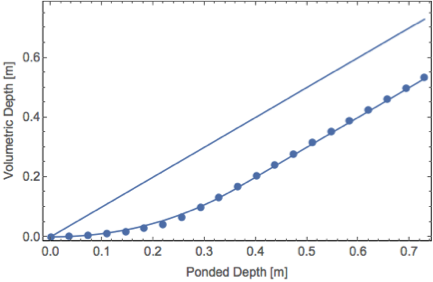
\includegraphics[width=6cm, height=6cm]{./figures/polygons-finescale/picture4.png}
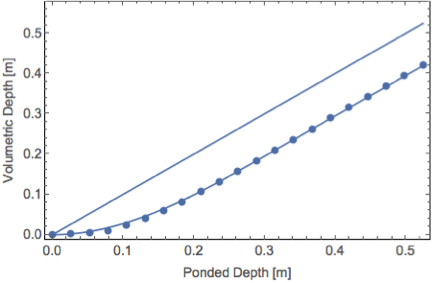
\includegraphics[width=6cm, height=6cm]{./figures/polygons-finescale/picture5.png}
\caption{Volumetric depth versus ponded depth for four additional ice-wedge polygons. \textbf{Should we include all of them??}}
\label{polygons}
\end{figure}

To calculate $\delta_\text{d}$ from the microtopography, we now propose an approach based on site percolation. Specifically, we fill the lowest elevation surface cells until the cluster of inundated cells spans the IWP. This is the percolation threshold. The water height at the percolation threshold defines the $\delta_\text{d}$. Figure~\ref{perc-cluster-poly40} shows the spanning cluster at the percolation threshold for the IWP of Figure~\ref{3Dpolygon40}. The depression depth calculated this way is 4.1 cm for this IWP.
It is reasonable to assume that the fractional conductance is well approximated by the fractional cross section available to flow, which can be estimated as the ratio of volumetric depth to ponded depth.

\begin{equation}
\Theta {(\delta_\text{d})} \approx \frac{( \Phi (\delta) - \Phi (\delta_\text{d}))} {\delta} H \left( \delta - \delta_\text{d}\right )
\end{equation}
Where $H$ is the Heaviside function. The numerator is the flowing cross sectional area. Note the velocity is multiplied by ponded depth to get a flux, so the molar flux appearing in the conservation equations becomes

\begin{equation}
\eta_{l} \delta U = - \eta_l  ( \Phi (\delta) - \Phi (\delta_\text{d})) H \left( \delta - \delta_\text{d}\right ) \Theta(\delta) \frac{(\delta - \delta_\text{d})^{2/3}}{n_\text{mann} (\| \nabla Z \| +\epsilon)^{1/2}} \nabla(Z + \delta)
\end{equation}
\begin{figure}
\centering
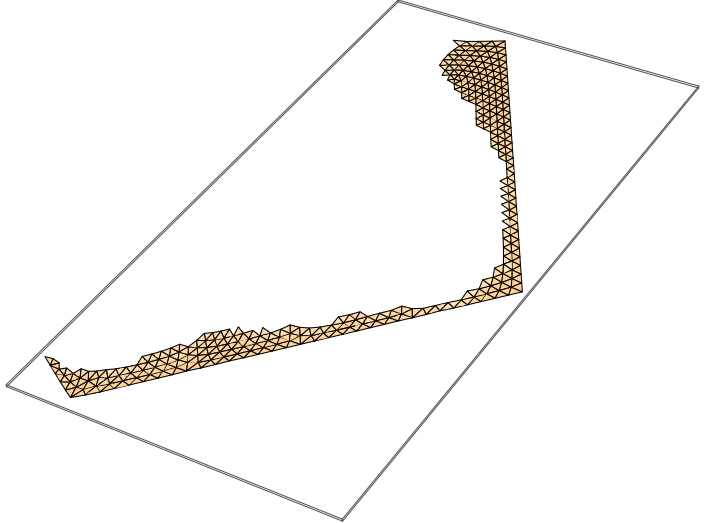
\includegraphics[width=12cm, height=6cm]{./figures/polygons-finescale/percolation-cluster-poly40.png}
\caption{The spanning cluster at the percolation threshold for the IWP of Figure~\ref{3Dpolygon40}. The water depth relative to the low point of the microtopography at the percolation threshold defines the depression depth.}
\label{perc-cluster-poly40}
\end{figure}

In summary, we hypothesize that the microtopographic effects on surface flow can be captured with a simple approximation with three parameters that can be computed from the microtopography:

\begin{itemize}
\item Subgrid relief $\delta_\text{max} = Z_{*,\text{max}} -   Z_{*,\text{min}}$, where  $Z_{*,\text{max}}$ and  $Z_{*,\text{min}}$ are the maximum and minimum elevation in the microtopography. 
\item Specific excluded volume $\delta_\text{ex}$, the soil volume above the microtopographic low point normalized by IWP area.
\item Depression depth $\delta$, the difference between the maximum and minimum elevation of the cells in the spanning cluster at the percolation threshold.
\end{itemize}
The subgrid releif and specific excluded volume come directly from the microtopography (univariate statistics). The depression depth requires a simple percolation algorithm to identify the spanning cluster at the percolation threshold. Values are given in Table~\ref{subgrid-para}.

\begin{center}
\begin{table}[htbp]
\caption{Parameters used in the subgrid model}\label{subgrid-para}
\begin{tabular}{| c |c|c|c|c|c|c|c|}
\hline
& C06 & C31 & C40 & C44 & C45 & A0 & B01 \\ \hline
 $\delta_\text{max}(m)$ & 0.404 & 0.262 & 0.483 & 0.364 & 0.350 & 0.361 & 0.411 \\ \hline
$\delta_\text{ex}(m)$ & 0.2 & 0.105 & 0.23 & 0.2 & 0.15 & 0.185 & 0.26\\ \hline
$ \delta_\text{d}(m)$ & 0.069 & 0.128 & 0.043 & 0.187 & 0.164 & 0.222 & 0.143 \\ \hline
\end{tabular}

\end{table}
\end{center}
\section{The Advanced Terrestrial Simulator (ATS)}\label{ATS}
Here we provide a very brief overview of the ATS for a reference, for more details about the software infrastructure we refer the reader to ~\cite{ecoon2016managing, ats-website}. A fully integrated surface/subsurface and snow distribution modeling capability implemented in ATS are available here~\cite{spainter2016integrated, atchley2015}. In addition, a mixed-dimensional modeling strategy, mainly designed for the simulations of low-relief permafrost-affected regions, can be found here~\cite{jan2017}. The ATS is a publically-available massively parallel computer code, an extended version of Amanzi (flow and reactive transport simulator; see~\cite{moulton2012high}), based on process management tool called Arcos. In ATS, a proces kernel (PK) refers to governing mathematical equations representing a particular (or coupled) physical process(es). Further, Multiprocess Coordinators (MPCs) are available to facilitate coupling amoung PKs. This framework allows to dynamically build a complex/coupled hierarchical model structure. The flexible extensibility feature of the Arcos framework allowed to easily implement our subgrid model and couple with the existing PKs.

\section{Numerical Results and Discussions}\label{numerical-tests}
\FloatBarrier
\subsection{Simulations}
To assess the accuracy of the numerical results of our subgrid model, we compare our results with fine-scale simulations. . the results of seven fine-scale ice-wedge polygons and no subgrid results. To point out, the entire fine-scale IWP is considered as one grid cell in the subgrid and no subgrid model -- the slope depends on the elevation of the corners of the fine-scale IWP. For demonstration purpose, we consider surface-only flow simulations. In our work, the seven ice-wedge polygon for fine-scale simulations are considered from Barrow Environmental Observatory (BEO) and illustrated in Figures~~\ref{polygon40} and \ref{IWP-finescale}. These polygons consist of low-center, high-center, with well established troughs (relatively uniform elevation across the trough) and obstructions in the troughs, and hence represent a broader class of polygonal landscape. Three sets of numerical results of the subgrid model are presented:

%We also show that the subgrird model results are more closer than the no subgrid model the no subgrid simulations under-esitmate the water content. 
\begin{description}\itemsep0pt \parskip0pt
\item [Study I:] Subgrid uncalibrated results;
\item [Study II:] Subgrid results with calibrated values of the depression depth listed in Table~\ref{subgrid-para};
\item [Study III:] Subgrid simulations with calibrated values of the depression depth and a drag coefficient (Study II with drag factor).
\end{description}

Study II is motivated by fine-scale simulations, higher depression depth may delay breakthrough, and would lead to more accumulation of water in the depressions. That said, in Study II we adjust the value the depression depth computed by the percolation algorithm to provide a better fit to the fine-scale results. The process of adjusting model's parameters to replicate the benchmark (e.g., fine-scale computational or real experiments) results is known as calibration. Moreover, higher pressure in the subgrid model affects the overland conductivity and hence the discharge rate. To mimic the behavior of the fine-scale at the time of breakthrough and the recession period, the surface roughness is decreased by raising the manning coefficient in the governing equation. This analysis proposed Study III. Raising the manning coefficient is analogous to introducing a drag factor.

Numerical simulations are performed for a  ``pulse numerical test" scenario -- injection followed by recession. In other words, we start with a fully dry surface, and inject water at a constant rate at the inlet boundary until breakthrough happens (prescribed flux boundary for a certain period of time), then stop the water supply and let water pass through the outlet (free drainage boundary). The arrows shown in Figure~\ref{IWP-finescale} indicate the inlet and outlet boundaries. The rainfall events are not considered. The presence of depression depth parameter in the flow law of our subgrid model will not allow to replicate the shape of the hydrograph because the fine-scale simulations will show immediate breakthrough. To capture such a behavior it would be more practical to determine the value of the depression depth dynamicly -- change the depression depth as the ponded depth changes.

\begin{figure}[!htb]
\centering
\vskip -1cm
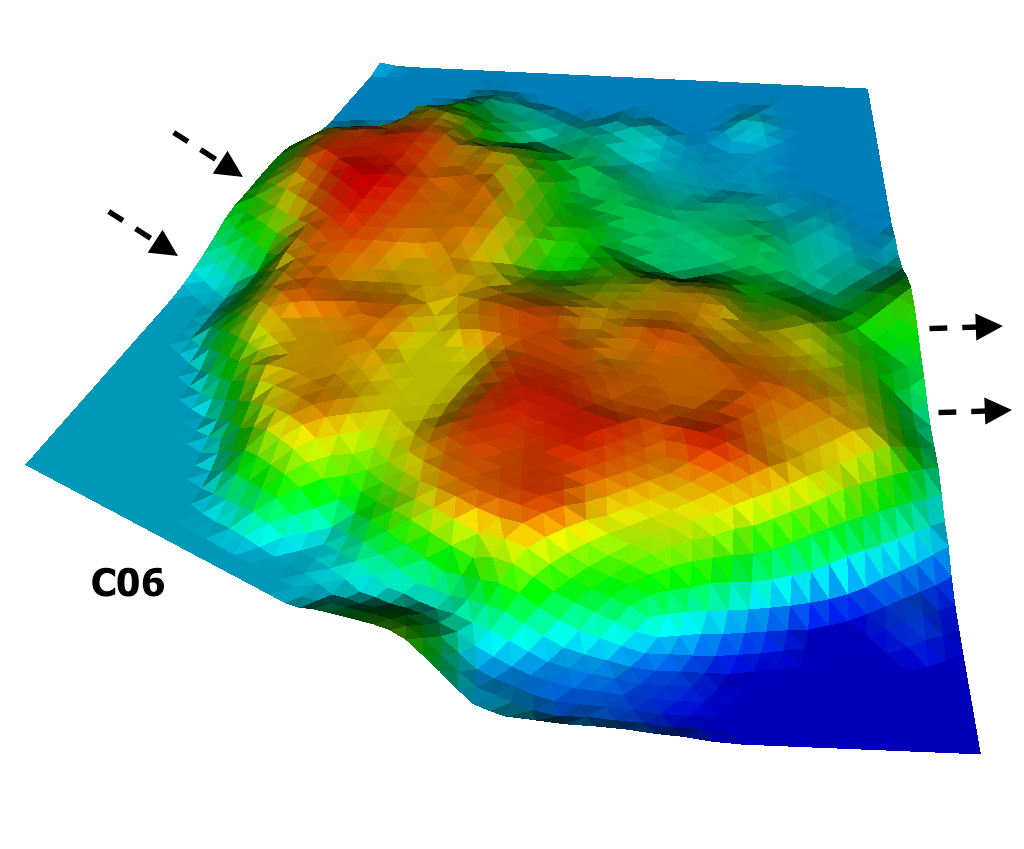
\includegraphics[width=6.2cm, height=6cm]{./figures/polygons-finescale/3Dpolygon06-3B.png}
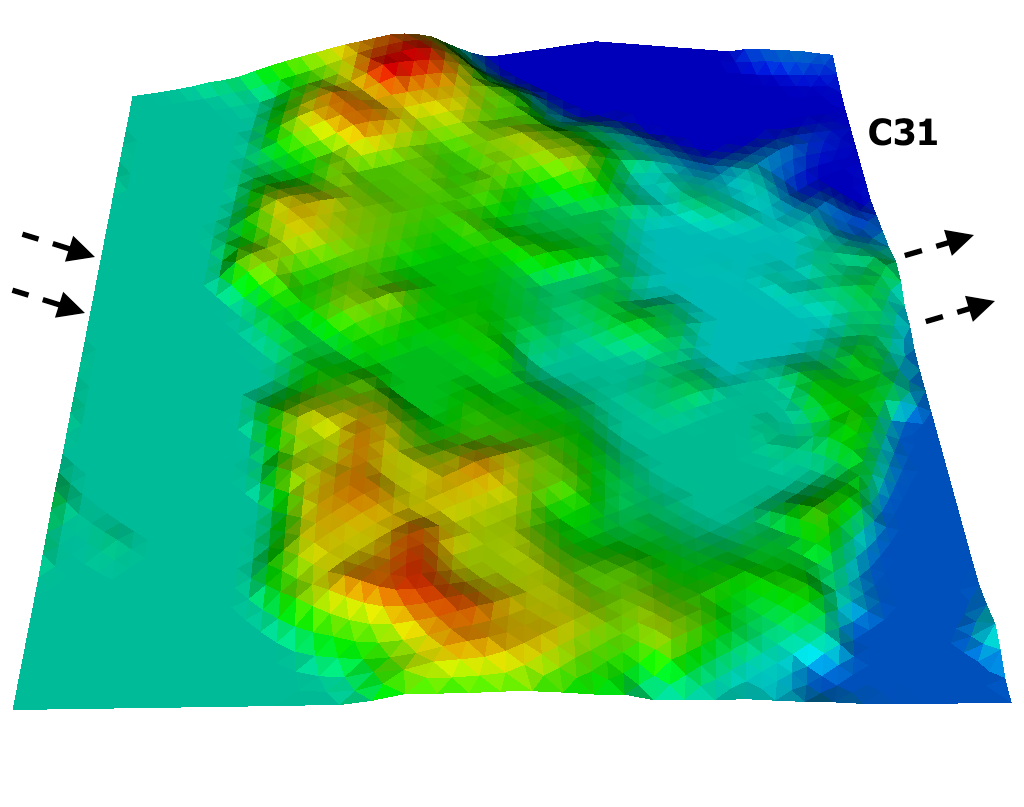
\includegraphics[width=6.2cm, height=6cm]{./figures/polygons-finescale/3Dpolygon31-3B.png}\\
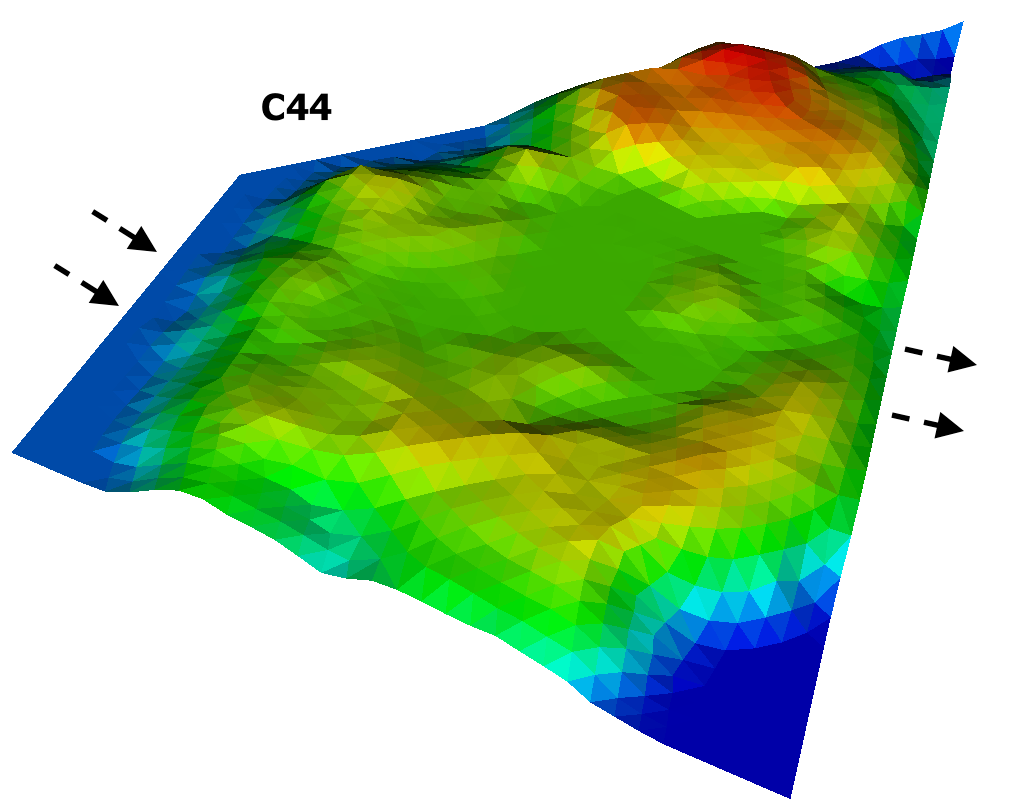
\includegraphics[width=6.cm, height=6cm]{./figures/polygons-finescale/3Dpolygon44-3B.png}
\hskip -0.4cm 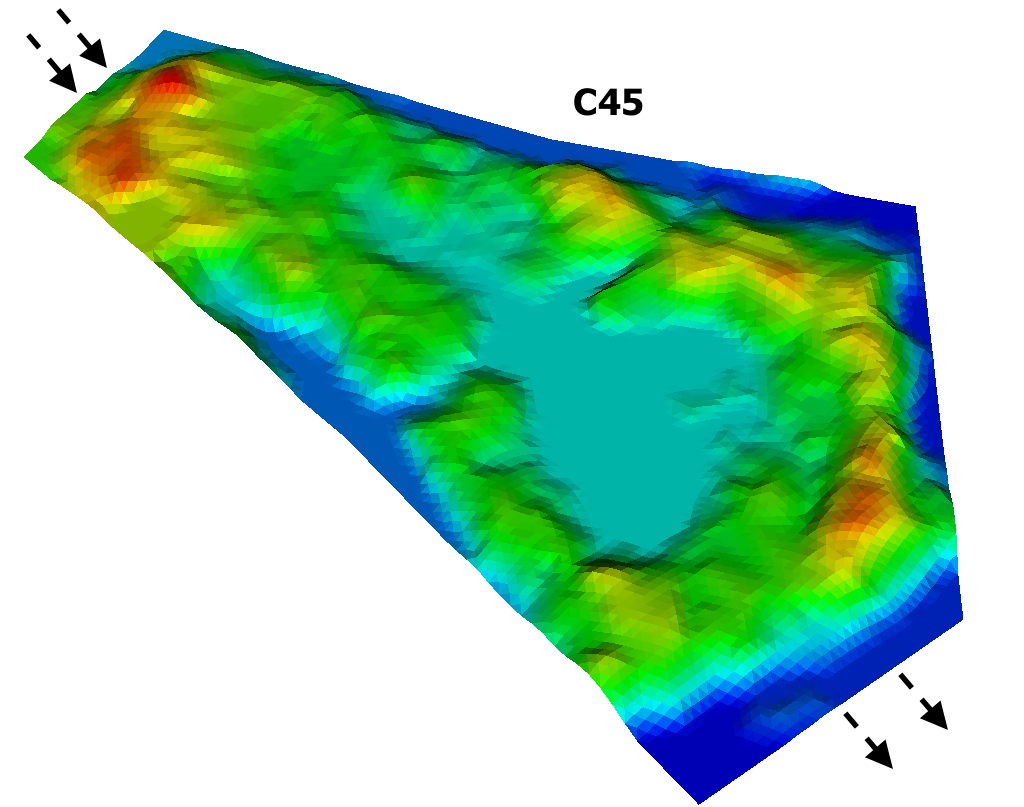
\includegraphics[width=6.8cm, height=6cm]{./figures/polygons-finescale/3Dpolygon45-3B.png}\\
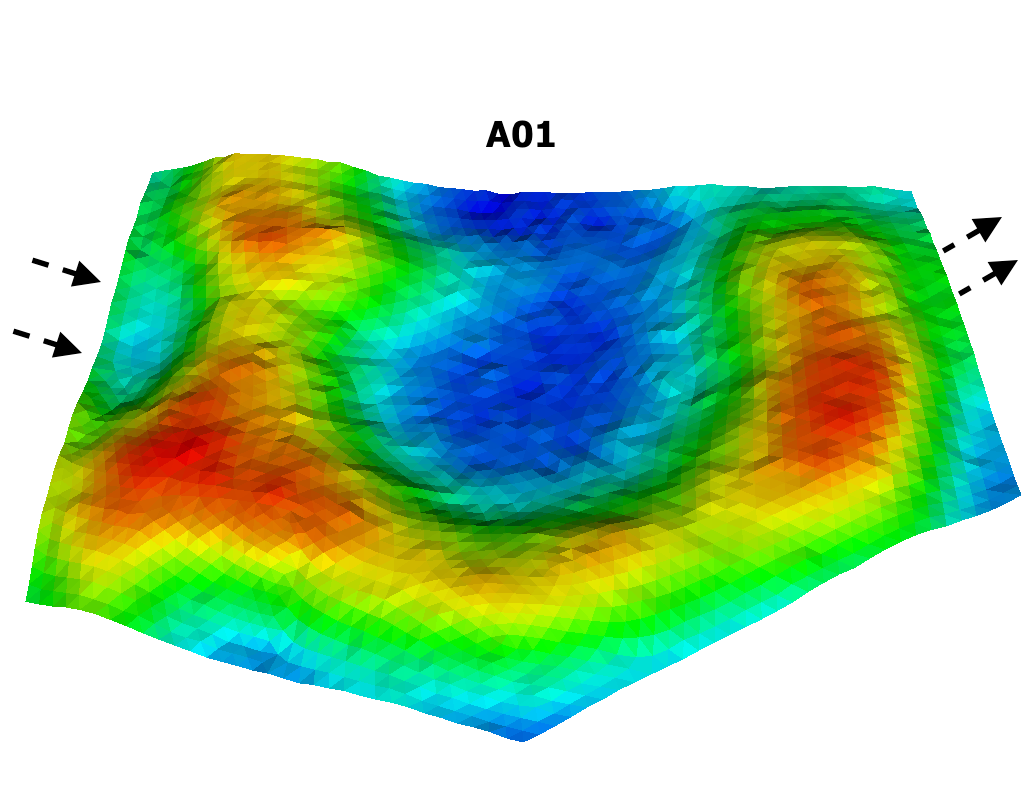
\includegraphics[width=6.2cm, height=6cm]{./figures/polygons-finescale/3DpolygonA01-3B.png}
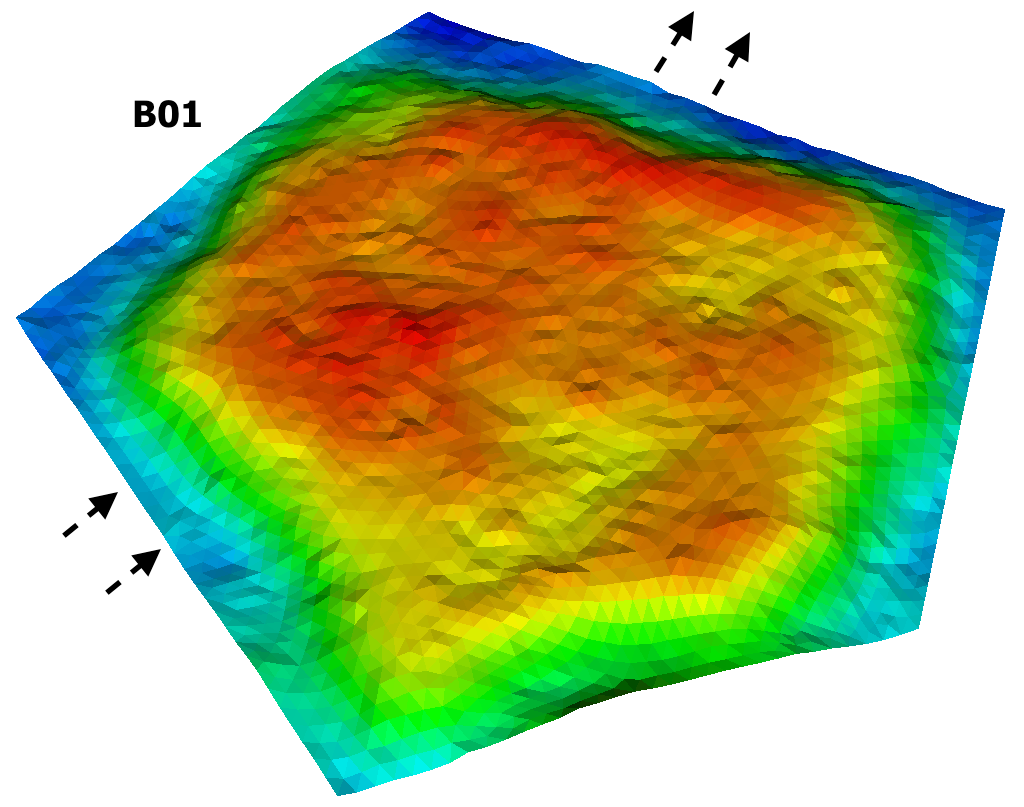
\includegraphics[width=6.2cm, height=6cm]{./figures/polygons-finescale/3DpolygonB01-3B.png}
\caption{An Illustration of the microtopography for ice-wedge polygons from Barrow Environmental Observatory (BEO). Red and dark blue spots correspond to high- and low-elevated regions. The arrows indicate inlet and outlet boundaries.}
\label{IWP-finescale}
\end{figure}
\FloatBarrier
\subsection{Results and Discussions}

Numerical results presented here correspond to the three studies mentioned above. We compare our results with fine-scale simulations of single IWPs, and we do not present any results on a cluster of fine-scale IWPs. We have carried out detailed simulations on all the polygons shown in Figure~\ref{IWP-finescale}, however, we discuss the results of polygon C44 in more detail and these results serve as a representative of all the remaining polygons as far as the accuracy and shape of the hydrographs are concerned. Figure~\ref{polygon-C44} compares the numerical results of the subgrid model with the fine-scale simulations, and no subgrid model of polygon C44. Clearly, Study I fails to match the fine-scale simulations, delayed breakthrough in the subgrid model is an indication of higher depression depth computed by the percolation algorithm; see Figure~\ref{polygon-C44}(a). Simulations with a calibrated depression depth, Study II, dramatically improve the shape of the hydrogragh and the water content in the system as highlighted in see Figure~\ref{polygon-C44}(b). However, a mismatch appears at the time of breakthrough and the beginning of the recession period even with the calibrated depression depth. As alluded to earlier, this is due to the huge head gradient between the center and the seepage face, and physically makes sense. Figure~\ref{polygon-C44}(c) illustrates the results of Study III, and it is evident that our subgrid model reproduces the fine-scale behavior, and the numerical results are identical.

\begin{figure}
\centering
(a) \hskip -.1cm  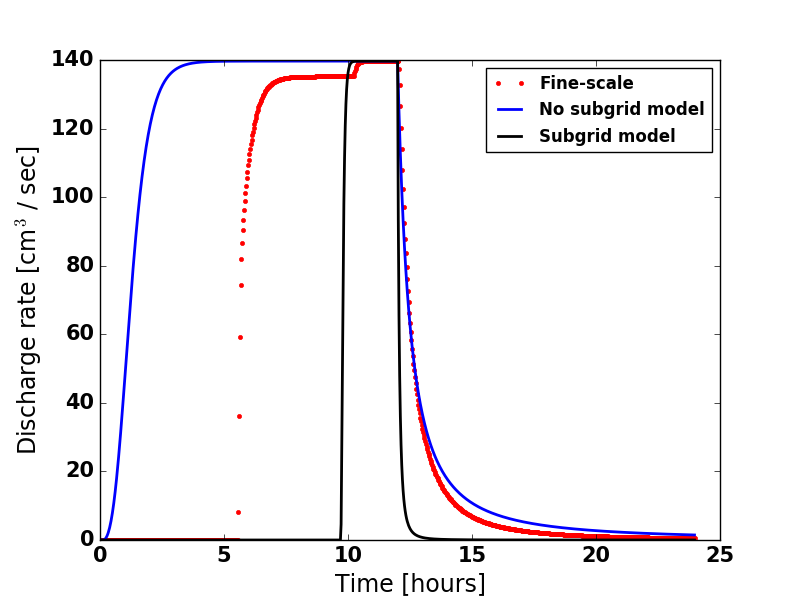
\includegraphics[width=6.cm, height=5.2cm]{./figures/POLYGON44/POLYGON44discharge.png}
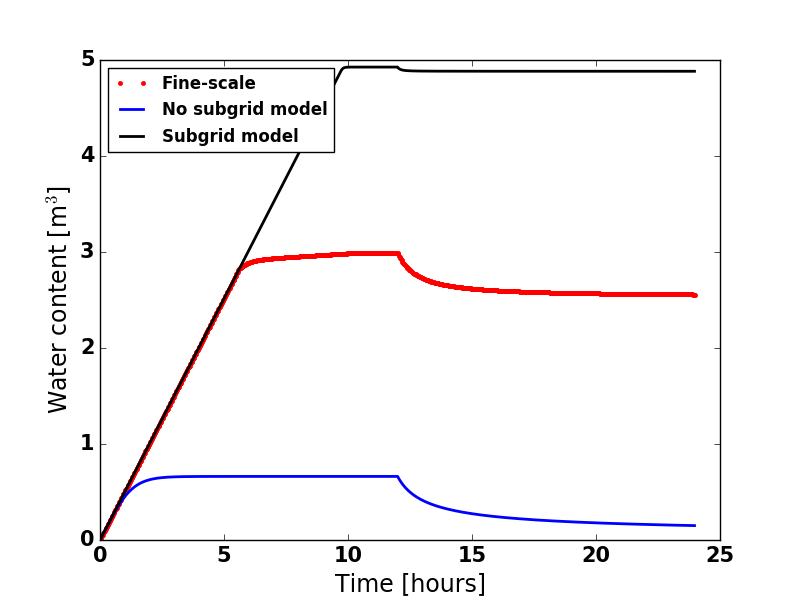
\includegraphics[width=6.cm, height=5.2cm]{./figures/POLYGON44/POLYGON44watercontent.png}\\
(b) \hskip -.1cm 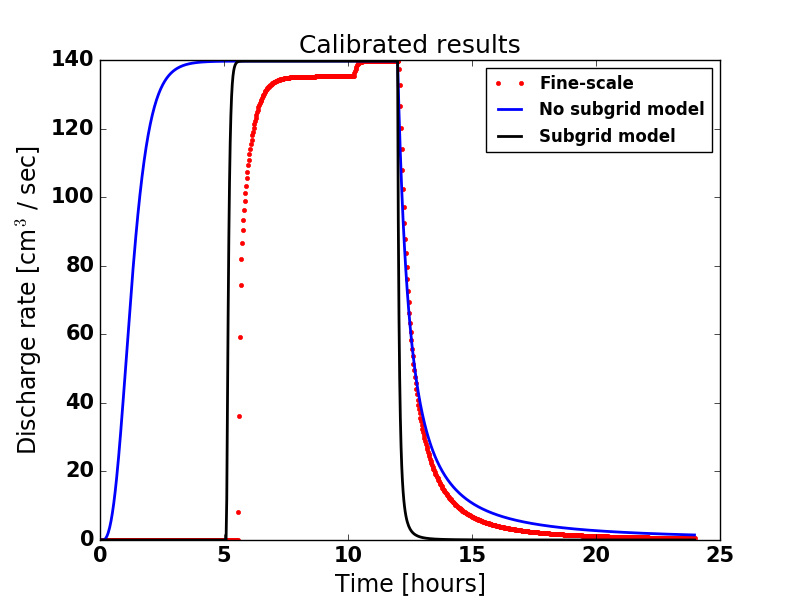
\includegraphics[width=6.cm, height=5.2cm]{./figures/POLYGON44/POLYGON44dischargeCalibDD.png}
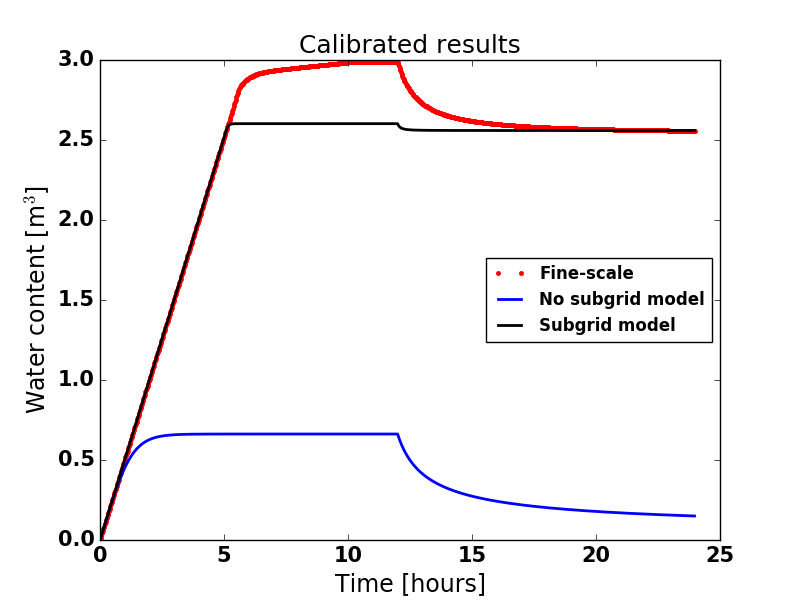
\includegraphics[width=6.cm, height=5.2cm]{./figures/POLYGON44/POLYGON44watercontentCalibDD.png} \\
(c) \hskip -.1cm 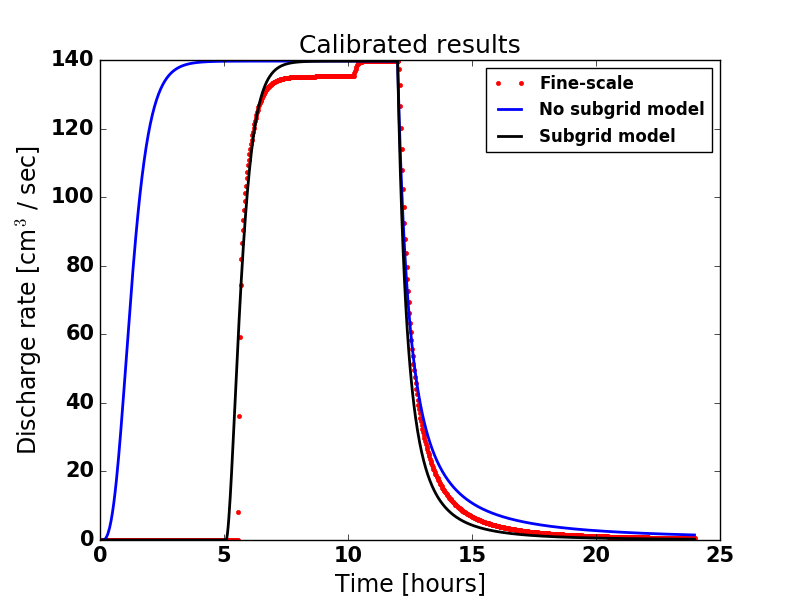
\includegraphics[width=6.cm, height=5.2cm]{./figures/POLYGON44/POLYGON44dischargeCalibDDManning.png}
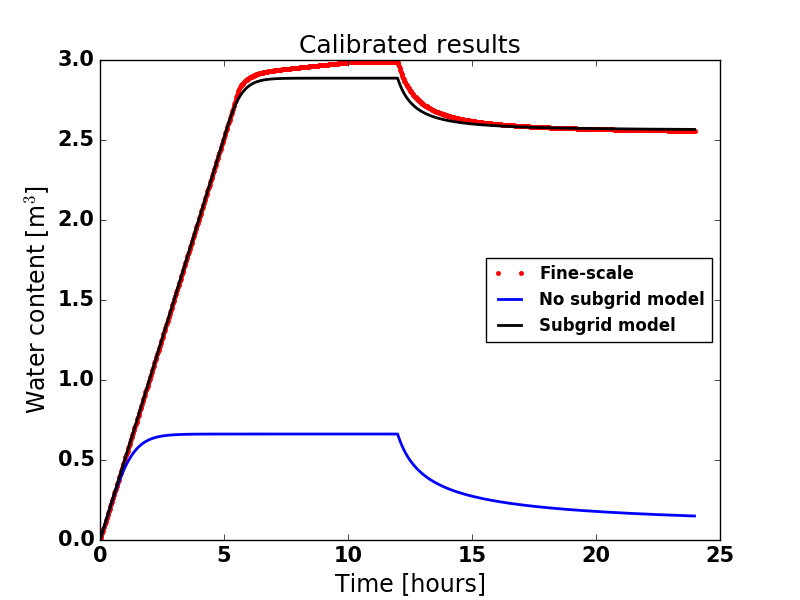
\includegraphics[width=6.cm, height=5.2cm]{./figures/POLYGON44/POLYGON44watercontentCalibDDManning.png}
\caption{(Polygon C44) Comparison of the numerical results of the subgrid model with the fine-scale and without subgrid model results. Rows (top to bottom) correspond to Study I, II and III, respectively.}
\label{polygon-C44}
\end{figure}

Figure~\ref{polygon-C06} compares the numerical results of Study I and III with the fine-scale and no subgrid model. The percolation algorithm computed the depression depth very accurately for polygon C06, and calibration (Study II) is not required. Similar to the results of polygon C44, the high overland conductivity in the subgrid model is reduced by increasing the surface roughness. It improves the results and replicate the recession period of the fine-scale results. It is important to see the amount of water (not available for drainage) in the system after the recession period. Figure~\ref{polygon-C06} also displays the water retained the in subgrid model and the fine-scale model -- the match is very close. 
For polygon C31, the results of the subgrid model are strongly affected by the depression depth in Study I, and lead to a mismatch. However, the results of Study II and III indicate that calibrated values of the depression depth and the surface roughness improved the simulated results dramatically and yield a close match as depicted in Figure~\ref{polygon-C31}. 
Numerical simulations correspond to polygons C31, C45, A01, and B01 are shown in Figures~\ref{polygon-C31}, \ref{polygon-C45}, \ref{polygon-A01}(a), and \ref{polygon-B01}, respectively. Overall, the results of the subgrid model are very encouraging and consistently yield a better fit to the fine-scale results as compared to the no subgrid model. 

\begin{figure}
\centering
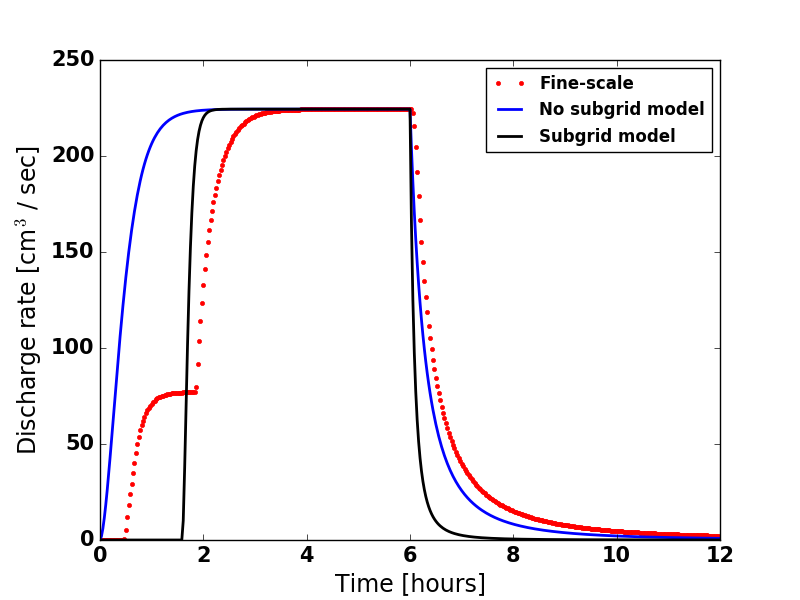
\includegraphics[width=6.2cm, height=6cm]{./figures/POLYGON06/POLYGON06discharge.png}
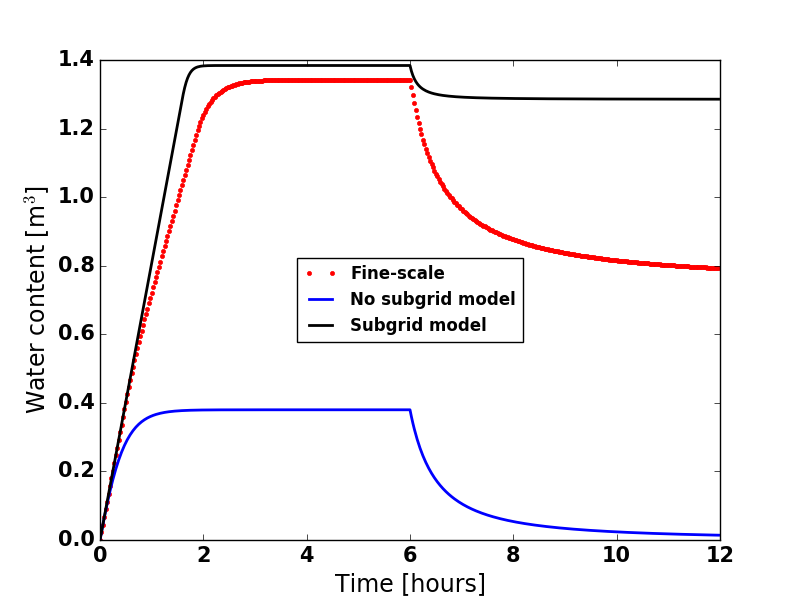
\includegraphics[width=6.2cm, height=6cm]{./figures/POLYGON06/POLYGON06watercontent.png}\\
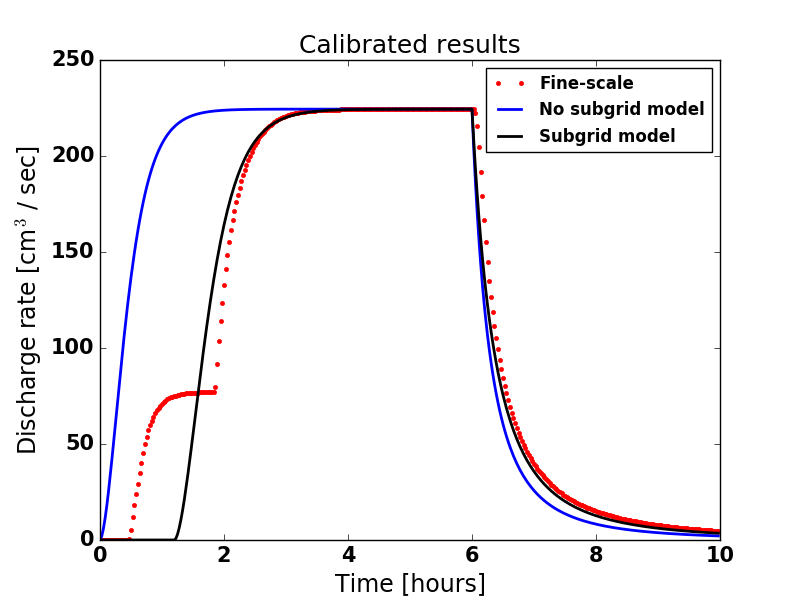
\includegraphics[width=6.2cm, height=6cm]{./figures/POLYGON06/POLYGON06dischargeCalibDDManning.png}
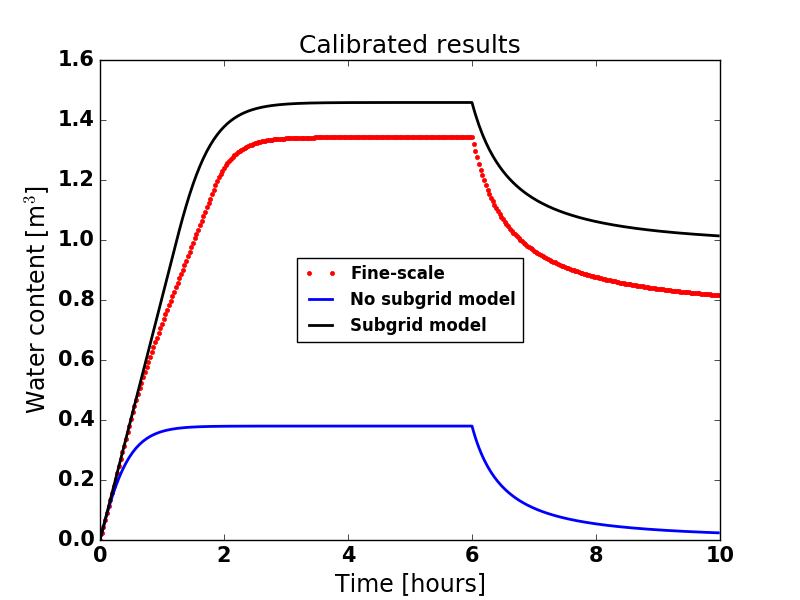
\includegraphics[width=6.2cm, height=6cm]{./figures/POLYGON06/POLYGON06watercontentCalibDDManning.png}
\caption{(Polygon C06) Comparison of the numerical results of the subgrid model with the fine-scale and without subgrid model results. Top and bottom row correspond to Study I and Study III, respectively.}
\label{polygon-C06}
\end{figure}


\begin{figure}
\centering
%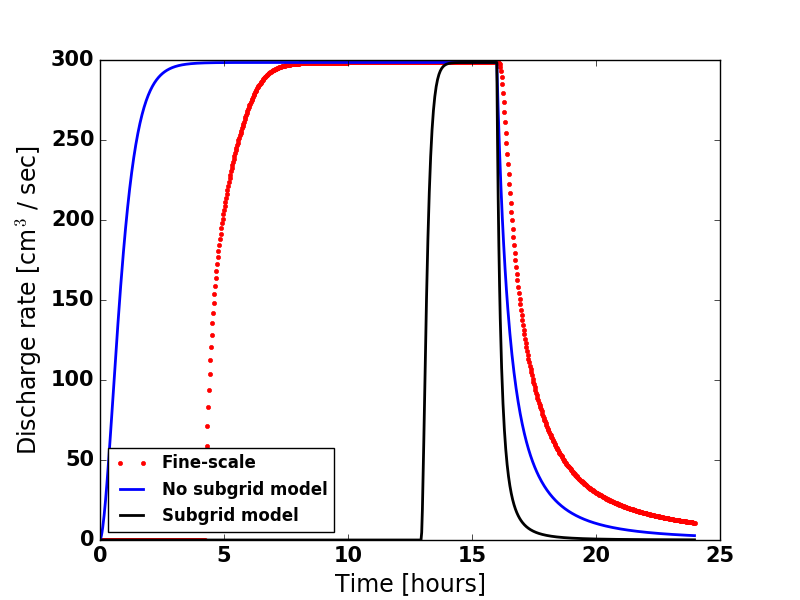
\includegraphics[width=6.2cm, height=5cm]{./figures/POLYGON31/POLYGON31discharge.png}
%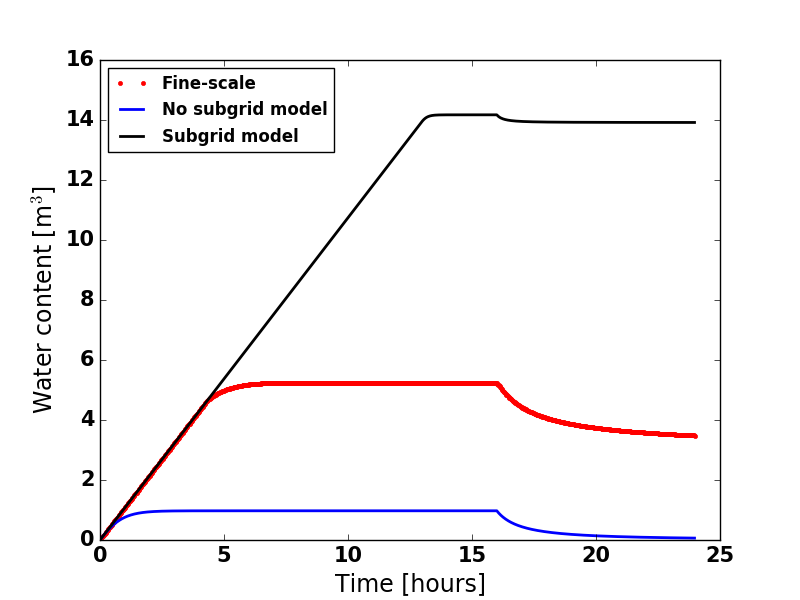
\includegraphics[width=6.2cm, height=5cm]{./figures/POLYGON31/POLYGON31watercontent.png}\\
%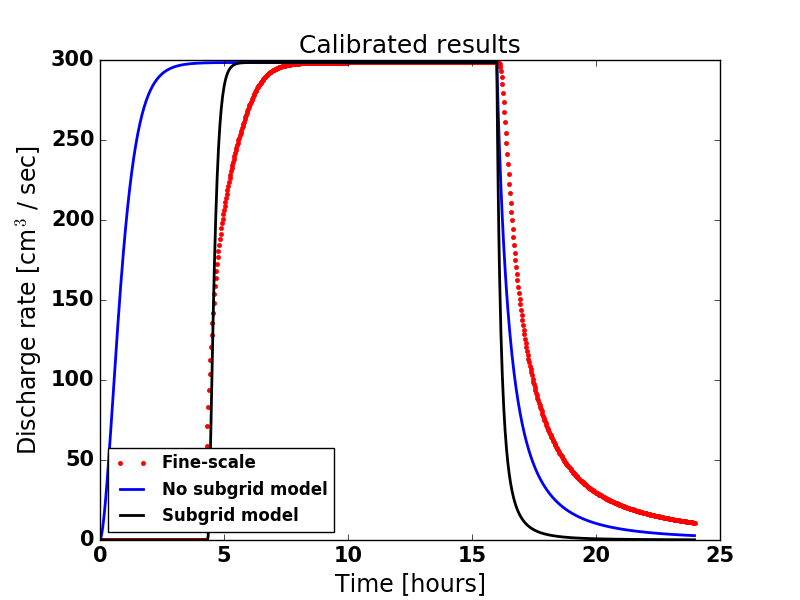
\includegraphics[width=6.2cm, height=5cm]{./figures/POLYGON31/POLYGON31dischargeCalibDD.png}
%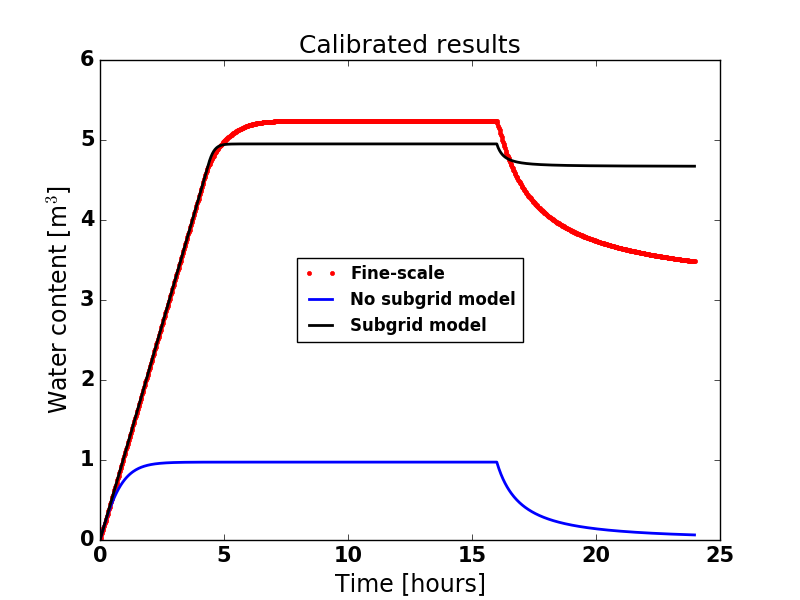
\includegraphics[width=6.2cm, height=5cm]{./figures/POLYGON31/POLYGON31watercontentCalibDD.png} \\
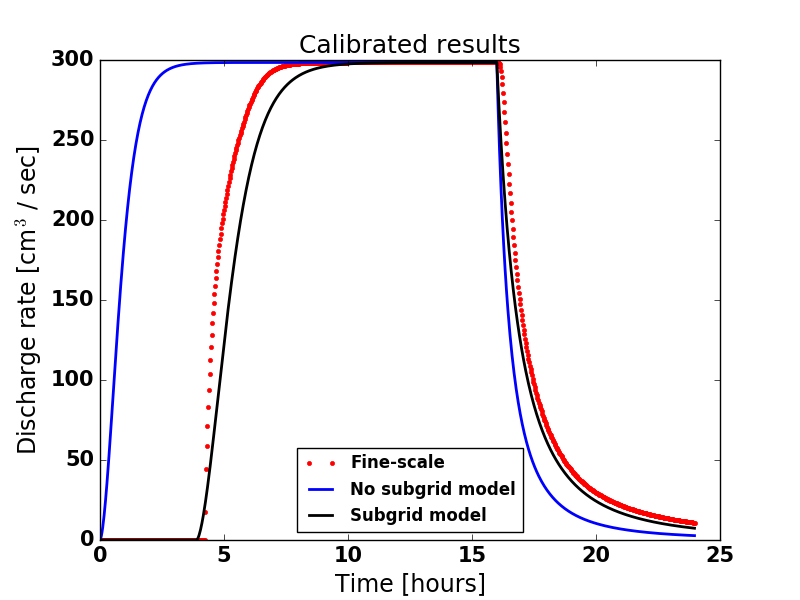
\includegraphics[width=6.2cm, height=5cm]{./figures/POLYGON31/POLYGON31dischargeCalibDDManning.png}
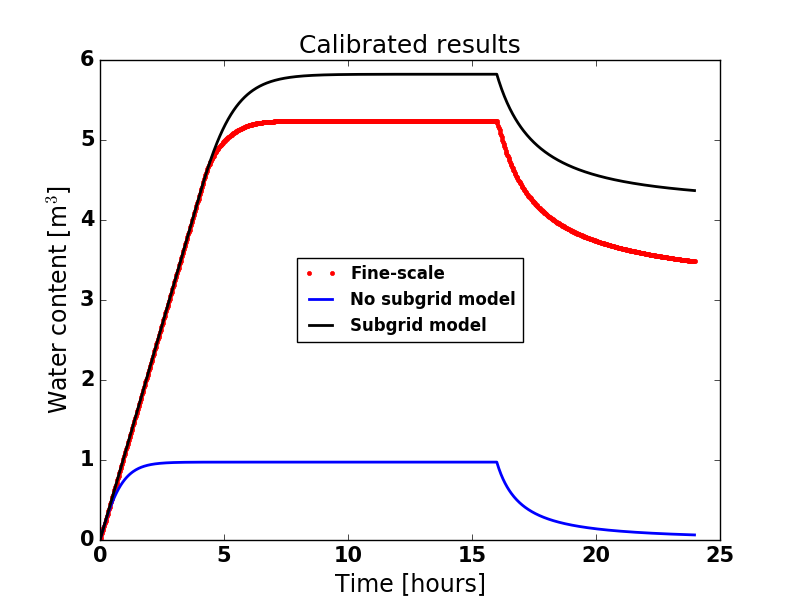
\includegraphics[width=6.2cm, height=5cm]{./figures/POLYGON31/POLYGON31watercontentCalibDDManning.png}
\caption{(Polygon C31) Comparison of the numerical results of the subgrid model with the fine-scale and no subgrid model. Results corresponded to Study III.}
\label{polygon-C31}
\end{figure}


\begin{figure}
\centering
%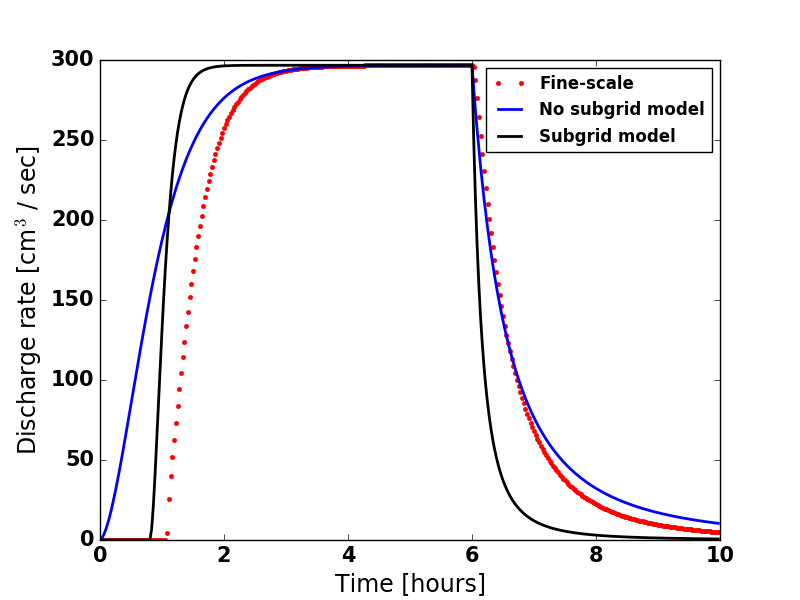
\includegraphics[width=6.2cm, height=5.5cm]{./figures/POLYGON40/POLYGON40discharge.png}
%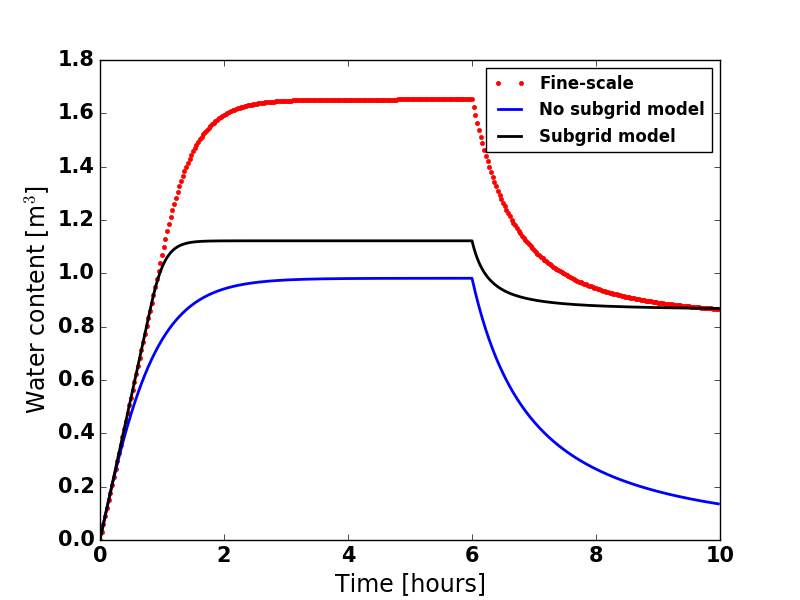
\includegraphics[width=6.2cm, height=5.5cm]{./figures/POLYGON40/POLYGON40watercontent.png}\\
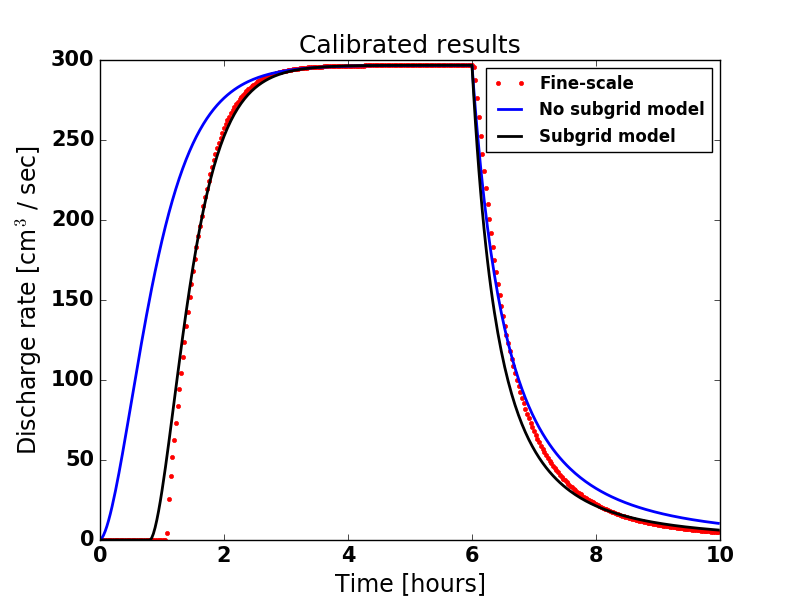
\includegraphics[width=6.2cm, height=5.5cm]{./figures/POLYGON40/POLYGON40dischargeCalibManning.png}
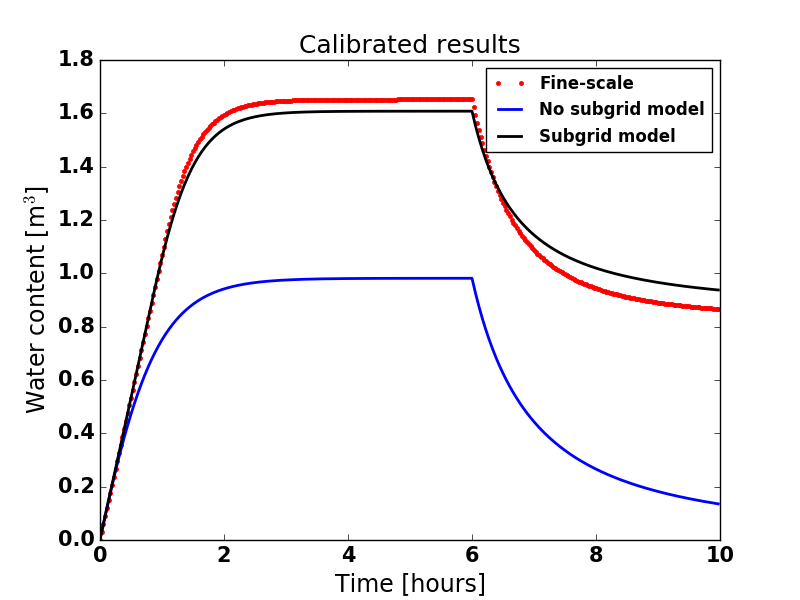
\includegraphics[width=6.2cm, height=5.5cm]{./figures/POLYGON40/POLYGON40watercontentCalibManning.png}
\caption{(Polygon C40) Comparison of the numerical results of the subgrid model with the fine-scale and without subgrid model results. Bottom row displays calibrated results.}
\label{polygon-C40}
\end{figure}




\begin{figure}[!h]
\centering
%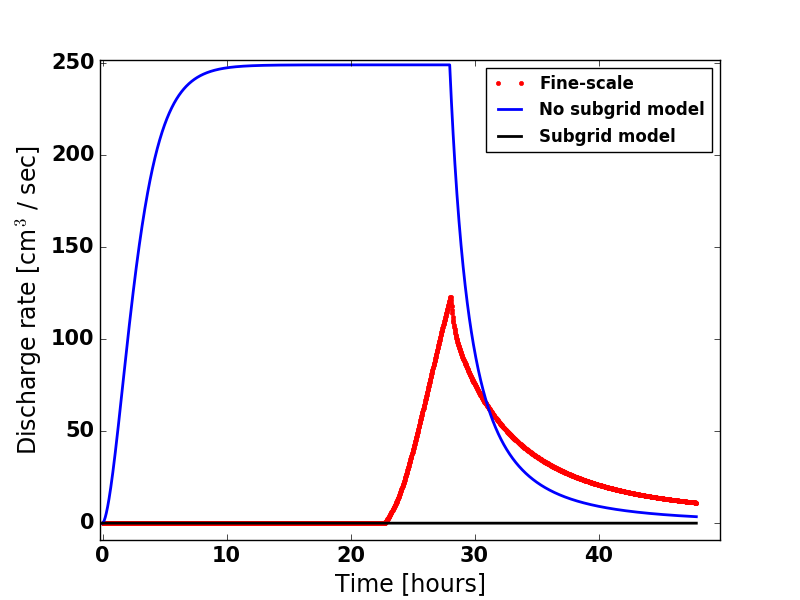
\includegraphics[width=6.2cm, height=5.5cm]{./figures/POLYGON45/POLYGON45discharge2.png}
%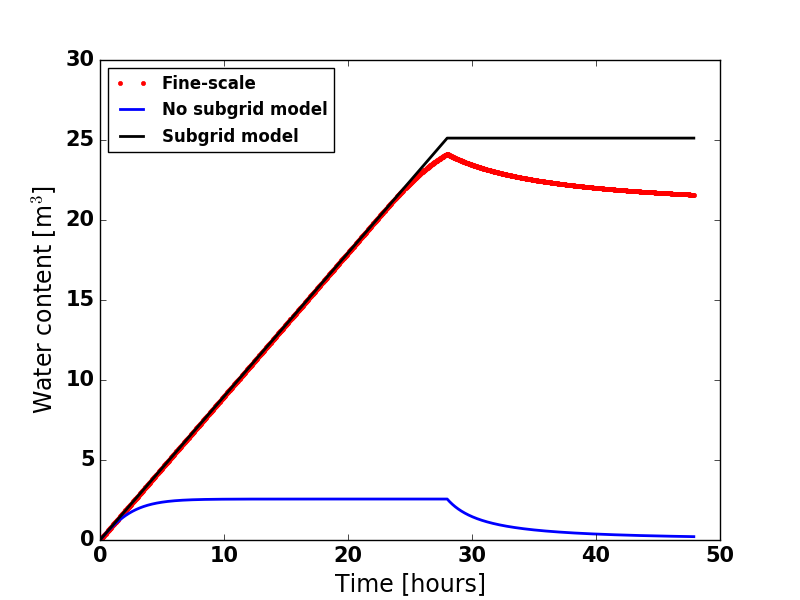
\includegraphics[width=6.2cm, height=5.5cm]{./figures/POLYGON45/POLYGON45watercontent.png}\\
%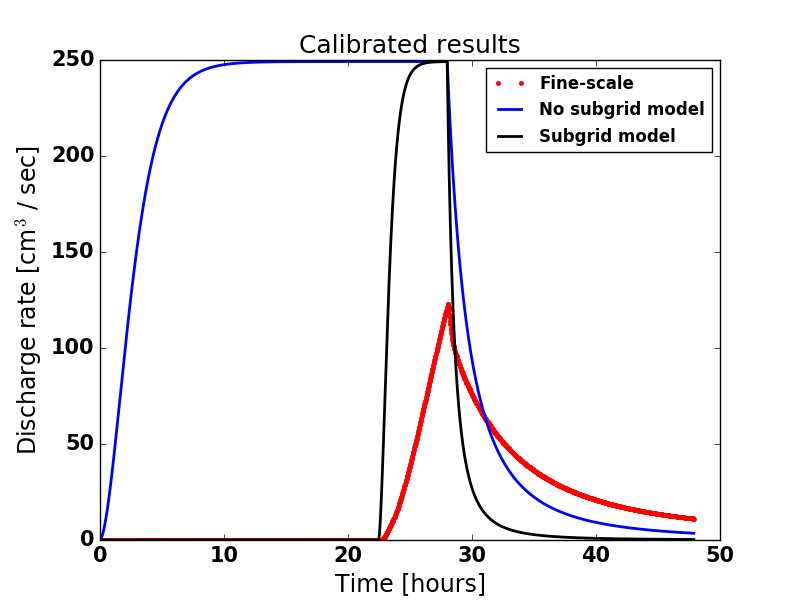
\includegraphics[width=6.2cm, height=5.5cm]{./figures/POLYGON45/POLYGON45dischargeCalibDD.png}
%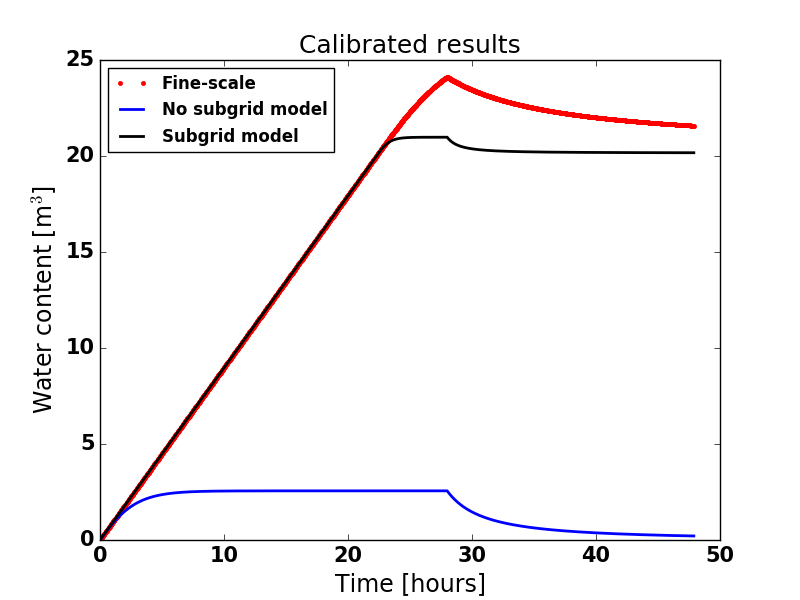
\includegraphics[width=6.2cm, height=5.5cm]{./figures/POLYGON45/POLYGON45watercontentCalibDD.png} \\
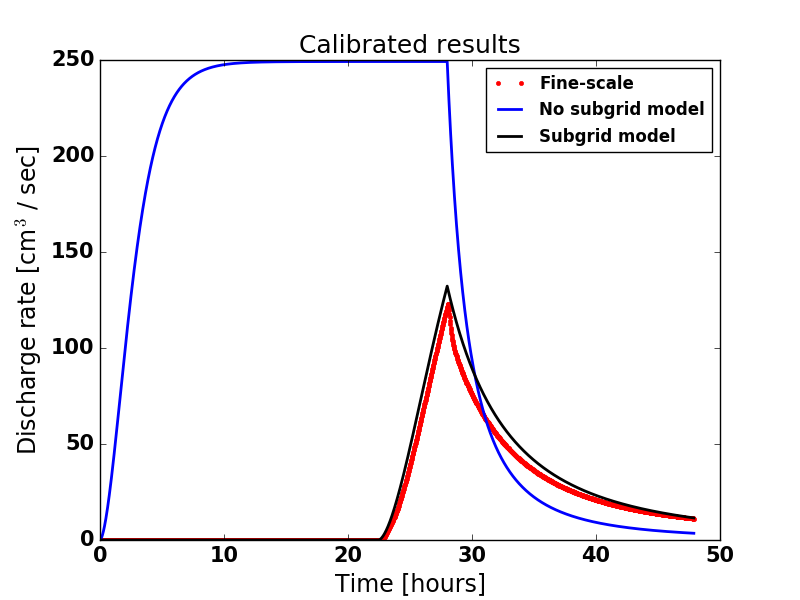
\includegraphics[width=6.2cm, height=5.5cm]{./figures/POLYGON45/POLYGON45dischargeCalibDDManning.png}
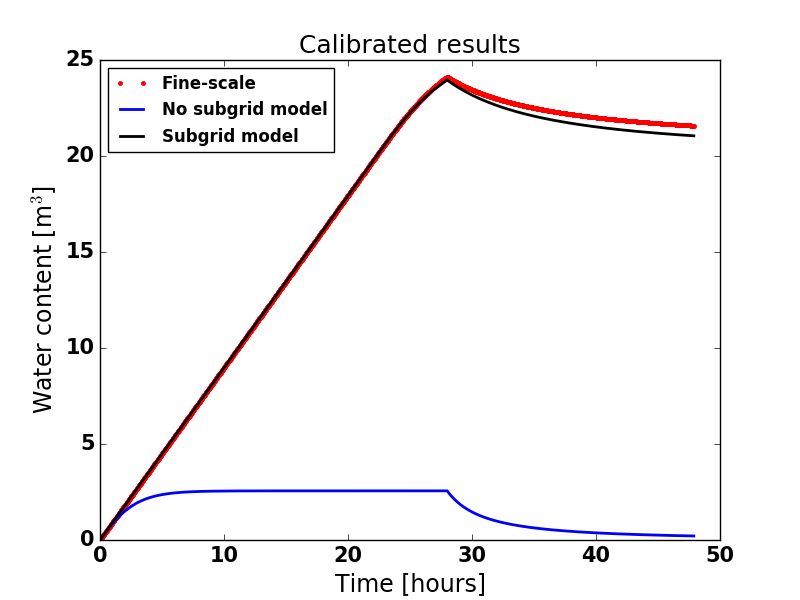
\includegraphics[width=6.2cm, height=5.5cm]{./figures/POLYGON45/POLYGON45watercontentCalibDDManning.png}
\caption{(Polygon C45) An illustration of the numerical results of the subgrid model, the fine-scale and no subgrid model. The simulations correspond to Study III.}
\label{polygon-C45}
\end{figure}




\begin{figure}[!h]
\centering
%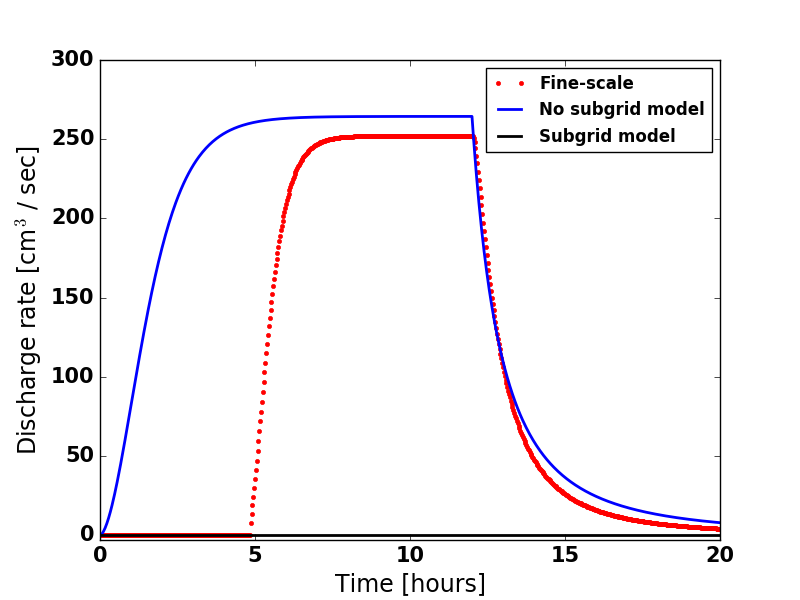
\includegraphics[width=6.2cm, height=5.5cm]{./figures/POLYGON_A01/POLYGON_A01discharge.png}
%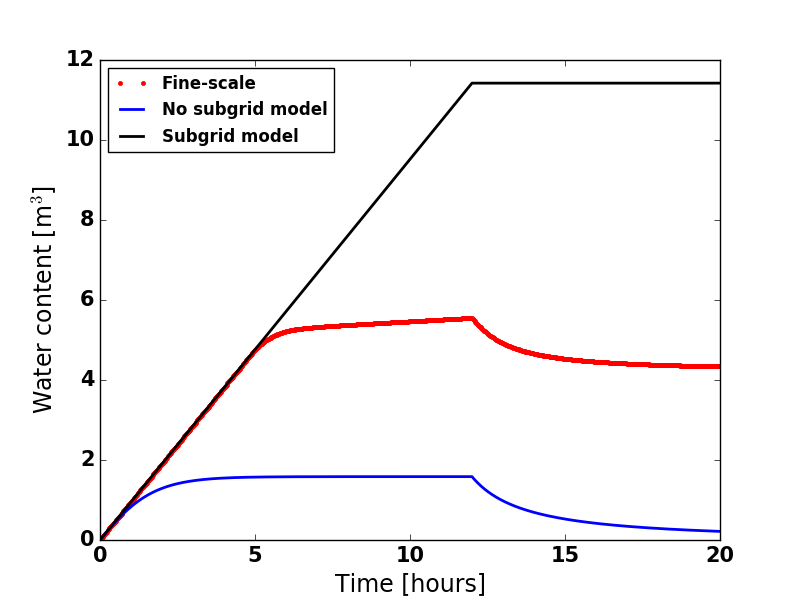
\includegraphics[width=6.2cm, height=5.5cm]{./figures/POLYGON_A01/POLYGON_A01watercontent.png}\\
%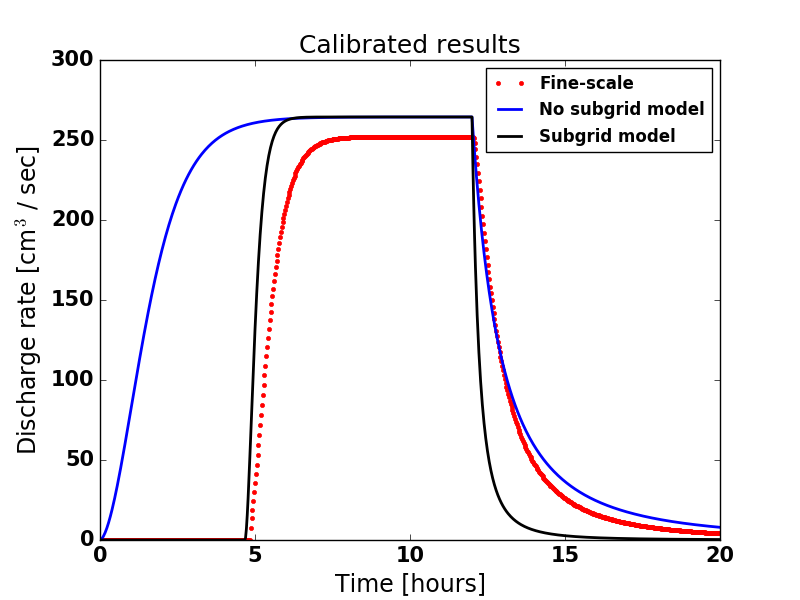
\includegraphics[width=6.2cm, height=5.5cm]{./figures/POLYGON_A01/POLYGON_A01dischargeCalibDD.png}
%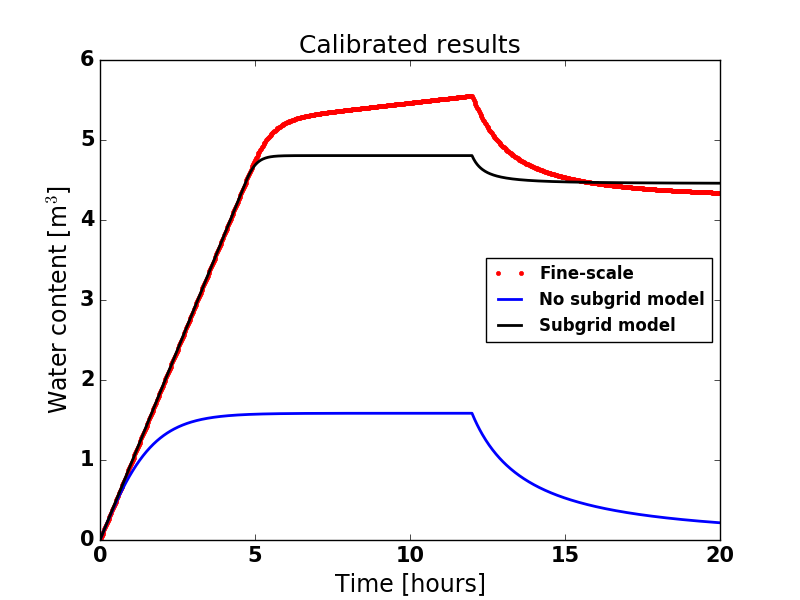
\includegraphics[width=6.2cm, height=5.5cm]{./figures/POLYGON_A01/POLYGON_A01watercontentCalibDD.png} \\
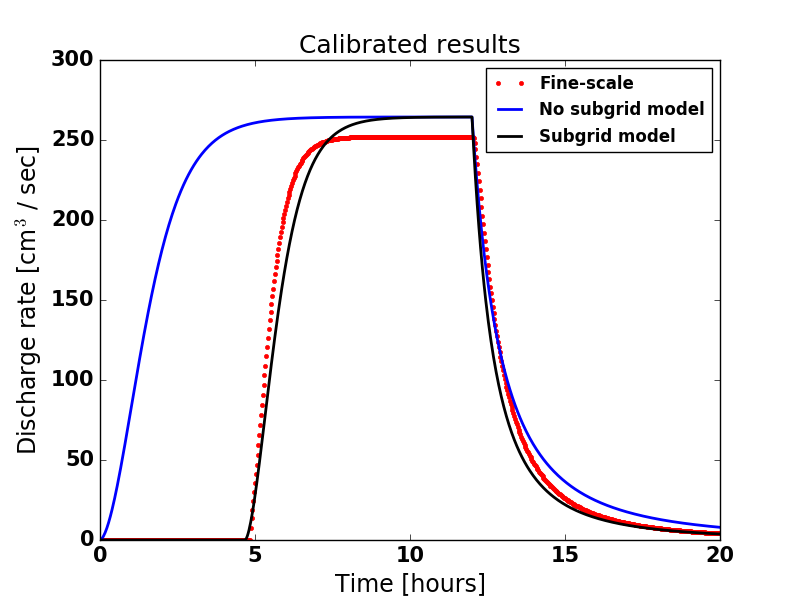
\includegraphics[width=6.2cm, height=5.5cm]{./figures/POLYGON_A01/POLYGON_A01dischargeCalibDDManning.png}
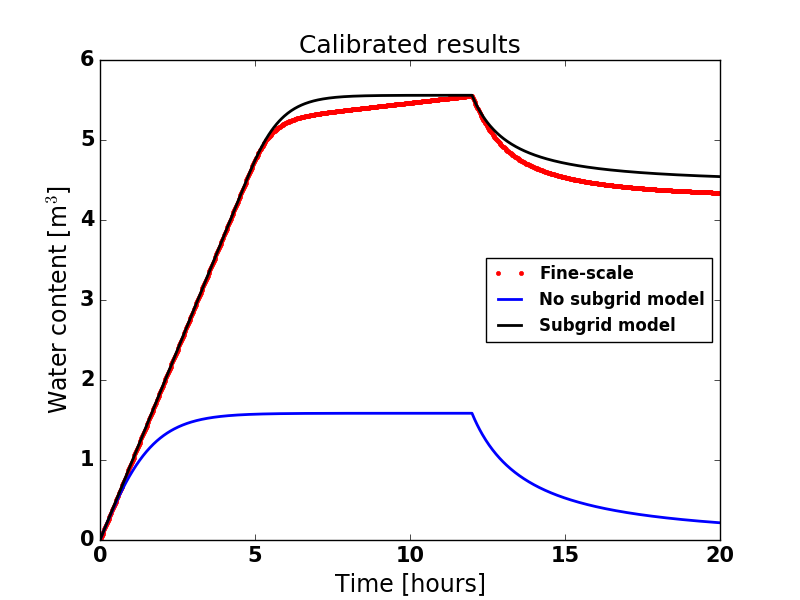
\includegraphics[width=6.2cm, height=5.5cm]{./figures/POLYGON_A01/POLYGON_A01watercontentCalibDDManning.png}
\caption{(Polygon A01) Comparison of the hydrographs and water content from the numerical simulation of the fine-scale, subgrid and no subgrid models. }
\label{polygon-A01}
\end{figure}



\begin{figure}[!h]
\centering
%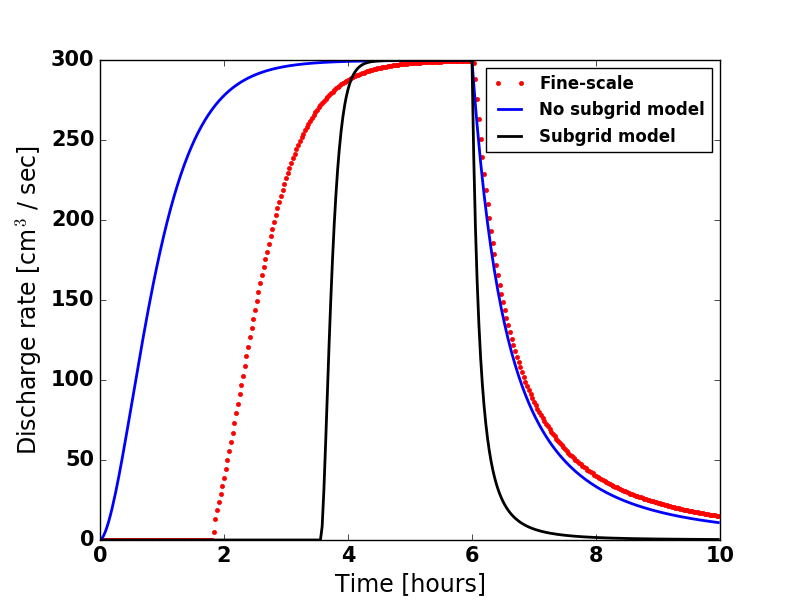
\includegraphics[width=6.2cm, height=5.5cm]{./figures/POLYGON_B01/POLYGON_B01discharge.png}
%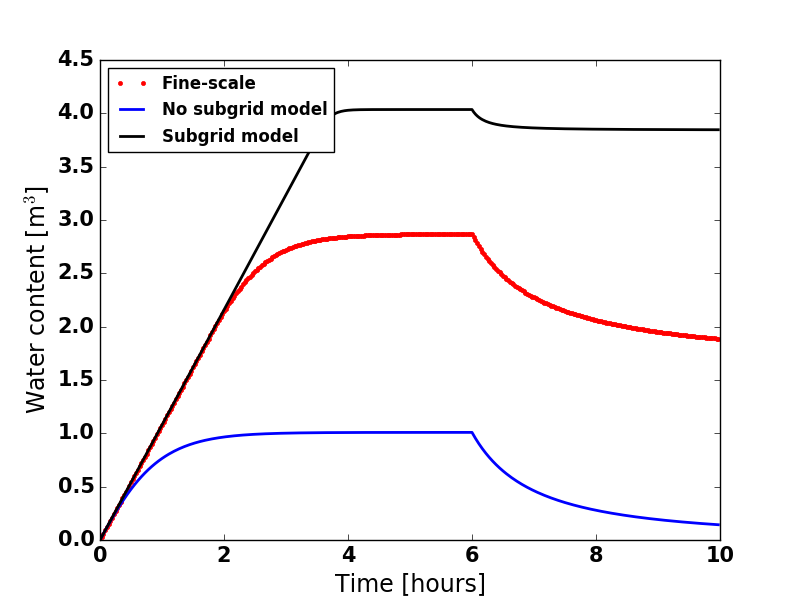
\includegraphics[width=6.2cm, height=5.5cm]{./figures/POLYGON_B01/POLYGON_B01watercontent.png}\\
%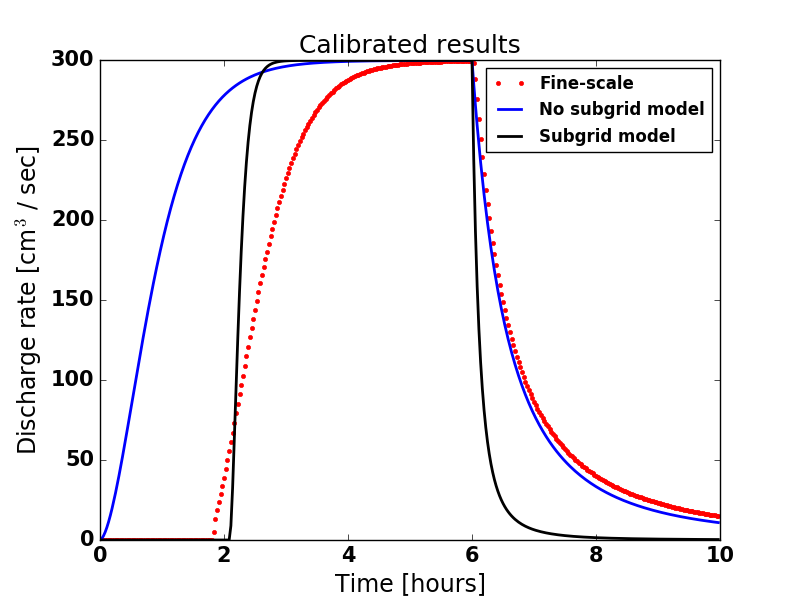
\includegraphics[width=6.2cm, height=5.5cm]{./figures/POLYGON_B01/POLYGON_B01dischargeCalibDD.png}
%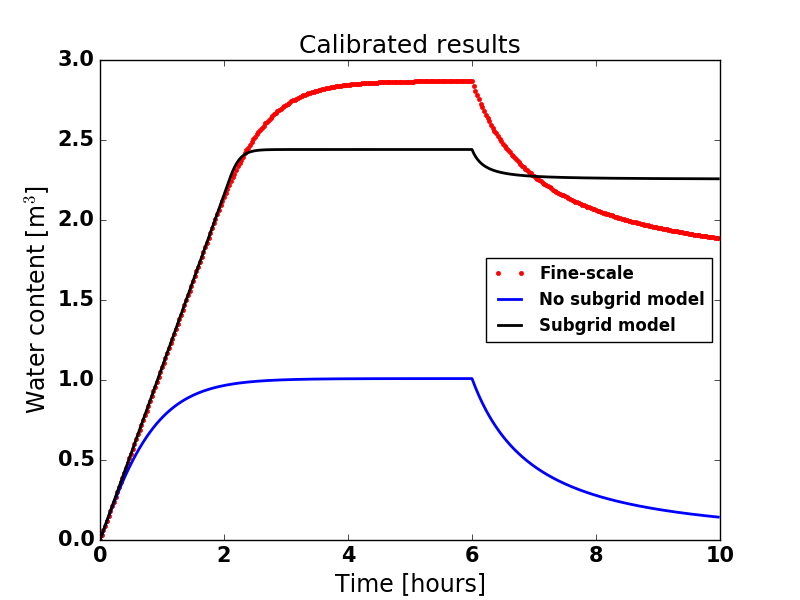
\includegraphics[width=6.2cm, height=5.5cm]{./figures/POLYGON_B01/POLYGON_B01watercontentCalibDD.png} \\
\includegraphics[width=6.2cm, height=5.5cm]{./figures/POLYGON_B01/POLYGON_B01dischargeCalibDDManning.png}
\includegraphics[width=6.2cm, height=5.5cm]{./figures/POLYGON_B01/POLYGON_B01watercontentCalibDDManning.png}
\caption{(Polygon B01) Comparison of the numerical results of the subgrid model with the fine-scale and without subgrid model results.}
\label{polygon-B01}
\end{figure}


\subsection{Additional Remarks}

\itemize{

\item Not surprisingly, the subgrid model favors high surface roughness that swings the results toward fine-scale simulations. A high agreement between the results of the subgrid model and fine-scale simulations due to reduced runoff is an indication of a needed drag coefficient in the flow law. A linear regression fit to the drag factor vs. the depression depth is depicted in Figure~\ref{curvefit-dd-manning}. The drag factor varies between zero and one, as the depression depth decreases the drag factor goes to unity -- a representation of flow over a flat surface. The fit indicates the resistance to flow increases with increasing depression.


\item For low-centered polygons such as C45 and A01, Study I (uncalibrated results) fails to match the hydrograph of the fine-scale simulations -- no breakthrough happens for the uncalibrated depression depths. Fine-scale simulations show that low-elevated regions may remain completely dry if they are not located in the main flow channel which trivial. However, as stated earlier, our percolation algorithm fills the lowest elevation cells until the cluster of inundated cells spans the IWP. Thereby, the direction of the injected fluid is important. For instance, considering polygon A01, the results are not comparable if the inlet and outlet are at sides inlet$_1$ and outlet$_1$, respectively. However, if the inlet and outlet are switched to inlet$_2$ and outlet$_2$ a desirable match is obtained; see Figure~\ref{polygon-A01-fig2}.

\item Application of invaded percolation (flow in the direction of least resistance) algorithm could provide more accurate depression depths, and would probably overcome the issue of calibrating parameters and/or location of inlet and outlet boundaries.

\item Most of our numerical experiments show that the subgrid model outperforms the no subgrid model even when the fine-scale flow behavior is not completely captured.

\item When the inlet boundary has obstructions (for example, polygon C06 in Figure~\ref{IWP-finescale}) and divides the incoming water into different flow channels, the water reaches the outlet boundary at different times and lead to a dual-peak (or may be multiple peaks) hydrograph.  Due to only one grid cell in the subgrid model, the dual-peak behavior is not possible to capture.

}
\begin{figure}[!h]
\centering
\includegraphics[width=6.cm, height=5.5cm]{./figures/fittedcurve-dd-1.png}
\includegraphics[width=6.cm, height=5.5cm]{./figures/fittedcurve-manning.png}
\caption{ (Left) Linear fitted-curve to the depression depth data. (Right) Drag factor vs. calibrated depression depth. \textbf{LEFT FIG. NEEDS TO BE UPDATED}}
\label{curvefit-dd-manning}
\end{figure}

\begin{figure}[!h]
\centering
(a)\includegraphics[width=6.cm, height=5.5cm]{./figures/POLYGON_A01/POLYGON_A01discharge.png}
\includegraphics[width=6.cm, height=5.5cm]{./figures/POLYGON_A01/POLYGON_A01watercontent.png}\\
(b)\includegraphics[width=6.cm, height=5.5cm]{./figures/POLYGON_A01/POLYGON_A01discharge-CalibDDManningTest3.png}
\includegraphics[width=6.cm, height=5.5cm]{./figures/POLYGON_A01/POLYGON_A01WC-CalibDDManningTest3.png}
%\includegraphics[width=6.2cm, height=5.5cm]{./figures/POLYGON_A01/POLYGON_A01dischargeCalibDDManning.png}
%\includegraphics[width=6.2cm, height=5.5cm]{./figures/POLYGON_A01/POLYGON_A01watercontentCalibDDManning.png}
\caption{(Polygon A01) An illustration of the choice of the inlet and outlet boundaries on the numerical results. The orientation affects the match between the fine-scale and subgrid model. (a) inlet$_1$ and outlet$_1$ boundary; (b) inlet$_2$ and outlet$_2$  boundary.}
\label{polygon-A01-fig2}
\end{figure}

%These results do not clearly indicate

\section{Conclusions}\label{conclusion}
The subgrid model presented in this paper is aimed at incorporating the microtopographic effects in the governing equations for the simulations at watershed-scale. The comparatively analysis of the subgrid results with the fine-scale IWP results reveal that our model has the potential to accurately represent fine-scale flow behavior at larger spatial scales. Numerical results of the subgrid model compare very well with the fine-scale simulations conducted on seven ice-wedge polygons. In addition, the model is applied to 468 polygons watershed and the results are physically consistent. More rigorous analysis is required to simultaneously capture both surface runoff and precipitation. Moreover, invaded percolation could reduce the load of parameters calibration.
\section*{References}

\bibliography{reference}

\end{document}



